\chapter{SIG Web Luziânia}
\label{cap:sigluziania}

\section{Introdução}

O SIG Web Luziânia é um SIG Web com a finalidade de gerenciar e visualizar  dados de serviços básicos da cidade de Luziânia, os quais são: educação, lazer, saúde e segurança. Além disso, organizar os dados em um banco de dados geográfico para que seja inserida a geometria da localização exata de cada serviço básico.

Em um primeiro momento, foi realizado a coleta de dados de todos os serviços. Essa coleta foi realizada através de dados disponibilizados pela prefeitura do município, dados públicos encontrados na Internet e através de conhecimento empírico da localização dos serviços coletados.

Os dados relacionados a educação são de escolas, faculdades e escolas técnicas, todas distribuídas no âmbito municipal, estadual, federal e privado. Através de gráficos é visualizado informações disponibilizadas pelo Ministério da Educação (MEC), com as notas das instituições de ensino nas avaliações do Exame Nacional do Ensino Médio (ENEM) e do Índice de Desenvolvimento da Educação Básica (IDEB).

Os dados sobre saúde são de hospitais e postos de saúde, contendo as especialidades médicas presentes em cada um dos hospitais ou postos de saúde. Os dados sobre lazer são de localidades que envolvem entretenimento, entre elas: praças, quadras poliesportivas, teatro, cinema, restaurante, e bares. Os dados sobre segurança são de delegacias, presídios, órgãos de justiça e batalhões policiais.

O SIG Web Luziânia foi desenvolvido usando apenas tecnologias livres para uso. O sistema foi desenvolvido na linguagem de programação C\#, junto com o \textit{framework} de desenvolvimento Web \textit{ASP.NET MVC}. No sistema é possível visualizar e interagir com os dados de uma maneira rápida e segura, além de ser possível a criação de novos dados. O sistema é totalmente acessível em dispositivos móveis, sendo possível a população do município acessar de qualquer lugar necessitando apenas de acesso à Internet.

\section{Aplicação dos Quatro Universos}

Nesta seção é descrito como foi aplicado a metodologia dos quatro universos no desenvolvimento do SIG Web Luziânia.

\subsection{Universo Ontológico}
\label{universo-ontologico}

Para o desenvolvimento de um SIG Web é necessário escolher as entidades a serem representadas, assim com a sua descrição. Uma geo-ontologia é um conjunto de conceitos e das relações semânticas e espaciais entre esses termos \cite{gisasp}. A primeira etapa de desenvolvimento do SIG Web Luziânia foi a construção de sua geo-ontologia. Os conceitos relacionados com o SIG Web Luziânia são de dois tipos:

\begin{itemize}
\item O primeiro tipo, envolve os conceitos associados às entidades não geográficas;
\item O segundo tipo, os conceitos associados às entidades geográficas criadas pelos seres humanos para representar entidades sociais e institucionais que descrevem entidades individuais criadas por ação e por leis. Essas entidades possuem uma identidade única e uma fronteira que as distinguem do mundo ao seu redor.
\end{itemize}
	
As entidades identificadas nesse cenário para o desenvolvimento do SIG Web Luziânia foram: 

\begin{itemize}
\item Usuário: pessoa responsável pelo controle dos dados do sistema;
\item Perfil: define o tipo de acesso do usuário ao sistema;
\item Cidade: localidade onde os dados serão georreferenciados;
\item Educação: localidades relacionadas as instituições de ensino;
\item Avaliação: avaliações escolares vinculadas as instituições de ensino;
\item Segurança: localidades relacionadas a segurança;
\item Tipo Segurança: tipo de localidade de segurança (delegacias, presídios, órgãos de justiça e batalhões policiais);
\item Lazer: localidades relacionadas ao entretenimento;
\item Tipo Lazer: tipos de localidades de entretenimento (praças, quadras poliesportivas, teatro, cinema, restaurante, e bares);
\item Saúde: localidades relacionadas a saúde;
\item Tipo Saúde: tipos de localidades de saúde (hospitais e postos de saúde);
\item Especialidade: especialidades médicas vinculadas as localidade de saúde.
\end{itemize}

\subsection{Universo Formal}

O paradigma dos quatro universos trata apenas do problema da representação computacional do espaço, por esse motivo será realizada apenas a passagem do universo ontológico para o universo formal das entidades geográficas do SIG Web Luziânia, ou seja, dos conceitos com características geográficas. Apenas os conceitos de educação, lazer, saúde e segurança possuem características geográficas no SIG Web Luziânia.

A passagem do universo ontológico para o universo formal caracteriza em representar um conceito genérico no qual é definido os atributos que caracterizam esse conceito e como pode-se medir o seu território. O processo de medida consiste em associar números ou símbolos a diferentes ocorrências de um mesmo atributo, a fim de que a relação dos números ou símbolos reflitam essas variações. Para medir os conceitos de educação, lazer, saúde e segurança do SIG Web Luziânia, foi utilizado a escala de medida nominal que classifica objetos em classes distintas, como rótulos que podem ser qualquer símbolos, como por exemplo, a cobertura do solo, que tem rótulos como floresta, área urbana e área agrícola.

O conceito das entidades educação, lazer, saúde e segurança foi medido a partir da presença de localidades caracterizadas e partir de cada entidade. Esse conceito é modelado no espaço absoluto porque a localização exata é fundamental para esses conceitos. Existem dois modelos formais para entidades geográficas no espaço absoluto: geo-campos e geo-objetos.

As entidades educação, lazer, saúde e segurança foram modelados como geo-objetos porque são entidades distintas e identificáveis, cada entidade é definida por uma fronteira.

\subsection{Universo Estrutural}

Para passar do universo formal para o universo estrutural é necessário relacionar cada tipo de entidade do modelo formal a estruturas de dados do universo estrutural. Para cada tipo de entidade do modelo formal, há diferentes possibilidades de uso de estruturas de dados.

Todas as entidades geográficas do SIG Web Luziânia (educação, lazer, saúde e segurança) utilizaram a estrutura vetorial ponto para representar as coordenadas das suas fronteiras, porque o ponto representa ocorrências ou localizações no espaço. No caso específico das entidades geográficas presentes no sistema, todas representam localizações.

\subsection{Universo de Implementação}

O SIG Web Luziâna foi desenvolvido na arquitetura cliente-servidor, ou seja, clientes requisitam serviços aos servidores que provem serviços, estando interligados entre si utilizando uma rede de computadores, nesse caso específico, a Internet. Ele é dividido em duas partes: a parte georreferenciada, principal funcionalidade do sistema, e a parte administrativa responsável pelo controle dos dados que alimenta a base de dados utilizada na primeira parte.

O SIG Web Luziânia possui um banco de dados geográfico que foi implementado no SGBD PostgreSQL utilizando a extensão espacial PostGIS. A alimentação dos dados é realizada na parte administrativa do sistema, através do preenchimento manual dos formulários existentes no sistema.

A visualização dos dados georreferenciados no mapa ocorre na integração da comunicação \textit{RESTful} e a biblioteca Javascript \textit{Leaflet}.

O sistema foi desenvolvido utilizando o \textit{framework} de desenvolvimento Web \textit{ASP.NET MVC}, juntamente com a linguagem de programação C\# e Javascript para realizar validações do sistema.

\section{Modelo de Dados}

A estrutura do banco de dados geográfico do SIG Web Luziânia foi definida a partir de dois modelos de dados: o conceitual e o lógico. O modelo conceitual fornece uma abstração mais alta dos dados, no nível de usuário. O modelo lógico, descreve como os dados serão armazenados no SGBD.
O modelo de dados OMT-G é o padrão definido pela INDE para modelagem de dados conceituais \cite{inde}. O modelo OMT-G foi utilizado para a criação do modelo conceitual, o qual foi abordado na seção \ref{modelo-omtg} deste trabalho. A Figura \ref{fig:DiagramaOMTG} apresenta o modelo OMT-G do SIG Web Luziânia e suas respectivas entidades identificadas. 

Para o entendimento dos relacionamentos entre as entidades, foi utilizado o conceito de entidades apresentados na seção \ref{universo-ontologico}. Na Tabela \ref{tabela-omtg} é visualizada a explicação para cada relacionamento do modelo OMT-G.

Para a criação do esquema do banco de dados do SIG Web Luziânia em um SGBD é necessário transformar o modelo conceitual em um modelo lógico. Essa transformação consiste no mapeamento do modelo OMT-G para o modelo relacional (MR) que representa os dados em um banco de dados como uma coleção de relações (tabelas). A Figura \ref{fig:ModeloER} apresenta o modelo conceitual do SIG Web Luziânia que foi criado a partir desse mapeamento. As chaves douradas e vermelhas, representam respectivamente as chaves primárias e estrangeiras.

\newpage

\begin{figure}[h]
\centering
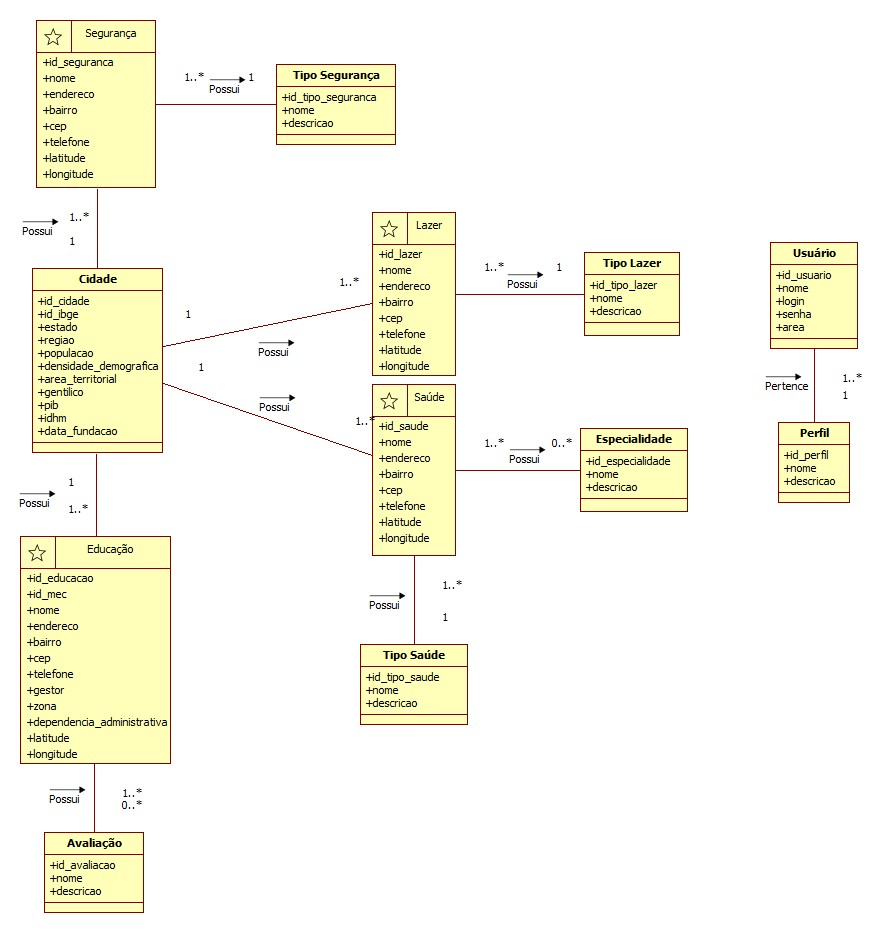
\includegraphics[width=0.69\textwidth]{./img/cap_IV/1-DiagramaOMTG}
\caption{Modelo OMT-G do SIG Web Luziânia.}
\label{fig:DiagramaOMTG}
\end{figure}

\begin{table}[htb]
\IBGEtab{
\caption{Explicação do modelo OMT-G do SIG Web Luziânia.}
\label{tabela-omtg}
}{
\begin{tabular}{ll}
\toprule
Relacionamento & Descrição\\
\midrule \midrule
Usuário e Perfil & Usuário pertence a um perfil, e um perfil pertence a vários usuários\\
\midrule
Cidade e Educação & Cidade possui instituições de ensino, instituições de ensino pertence a uma cidade\\
\midrule
Educação e Avaliação & Instituições de ensino possui uma avaliação ou várias, avaliação pertence\\
& a uma ou várias instituições de ensino\\
\midrule
Cidade e Segurança & Cidade possui localidades de segurança, localidades de segurança\\
& pertence a uma cidade\\
\midrule
Segurança e Tipo Segurança & Localidades de segurança possui um tipo específico, um tipo possui\\
& uma ou várias localidades de segurança\\
\midrule
Cidade e Lazer & Cidade possui dados de entretenimento, dados de entretenimento pertence a uma cidade\\
\midrule
Lazer e Tipo Lazer & Dados de entretenimento possui um tipo específico, um tipo possui\\
& um ou vários dados de entretenimento\\
\midrule
Cidade e Saúde & Cidade possui localidades de saúde, localidades de saúde pertence a uma cidade\\
\midrule
Saúde e Tipo Saúde & Localidades de saúde possui um tipo específico, um tipo possui\\
& uma ou várias localidades de saúde\\
\midrule
Saúde e Especialidade & Localidades de saúde possui uma especialidade ou várias, especialidade possui\\
& uma ou várias localidades de saúde\\
\bottomrule
\end{tabular}}{}
\end{table}

\newpage

\begin{figure}[h!]
\centering
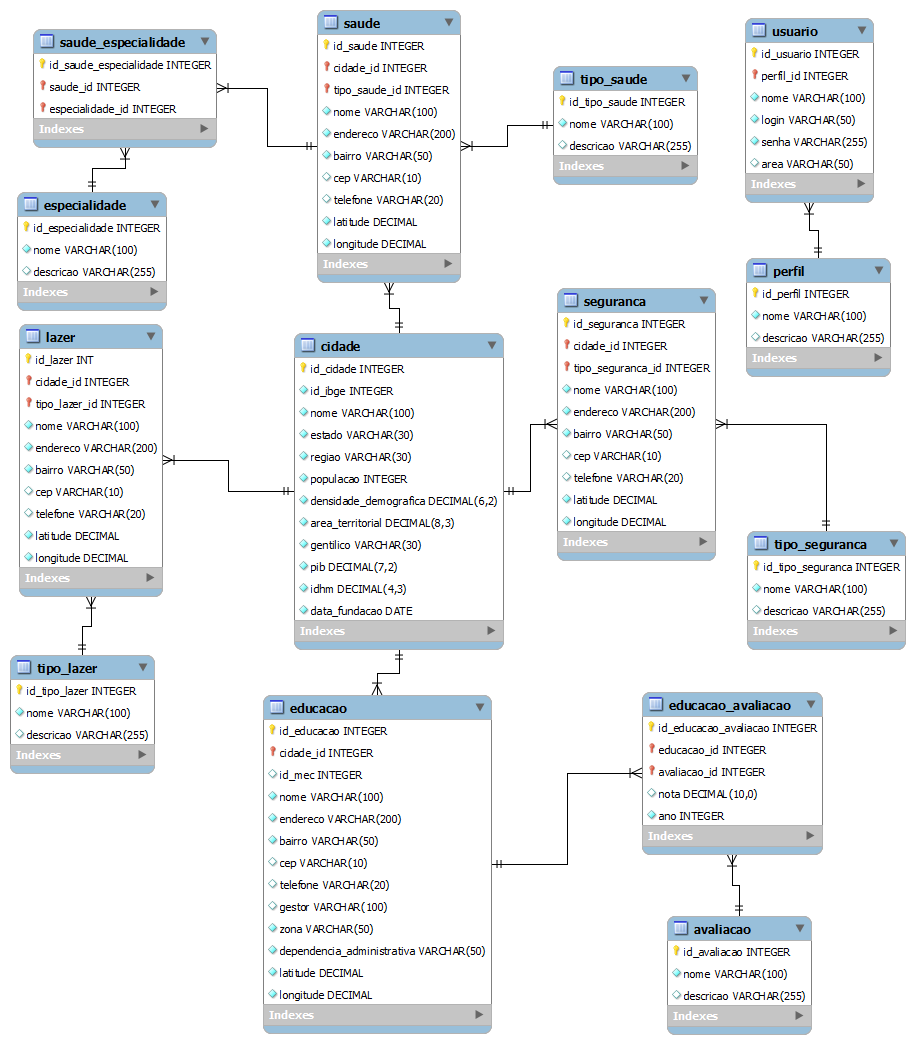
\includegraphics[width=0.75\textwidth]{./img/cap_IV/2-ModeloER}
\caption{Modelo relacional do SIG Web Luziânia.}
\label{fig:ModeloER}
\end{figure}

\section{Implementação}

Nesta seção é abordada questões relacionadas a implementação do SIG Web Luziânia, a arquitetura do sistema e as tecnologias utilizadas.

\subsection{Arquitetura do SIG Web Luziânia}

A arquitetura abstrata do SIG Web Luziânia é representada na Figura \ref{fig:arquiSig}, utilizando o tipo de arquitetura \textit{thick client} (definida no capítulo \ref{cap:sig}) e sendo composta por três grandes módulos: Camada de Interface, Camada de Aplicação e Camada de Persistência.

\begin{itemize}
\item A Camada de Interface é responsável pela interação do sistema com o usuário através de formulários e da visualização dos dados;
\item A Camada de Aplicação é responsável pelo mecanismo de gerar os dados do mapa;
\item A Camada de Persistência é responsável pelo tratamento e armazenamento dos dados em um SGBD.
\end{itemize}

\newpage

\begin{figure}[h]
\centering
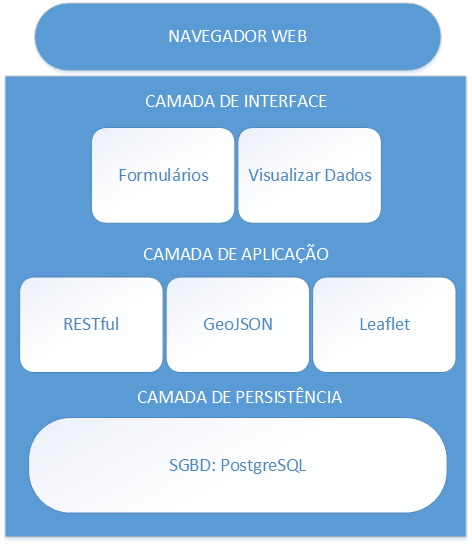
\includegraphics[width=0.55\textwidth]{./img/cap_IV/3-ArquiteturasSigLuziania}
\caption{Arquitetura abstrata do SIG Web Luziânia.}
\label{fig:arquiSig}
\end{figure}

O usuário interage com a Camada de Interface a partir de um navegador web. Ao acessar a página inicial do sistema, o usuário irá visualizar os dados georreferenciados plotados no mapa, além de visualizar esses dados com mais detalhes nos formulários apresentados na página inicial. A área administrativa do sistema possui formulários para inserção, visualização, atualização e deleção dos dados.

A camada de aplicação é responsável por gerar os dados que serão plotados no mapa. Essa camada é composta pelo sistema \textit{RESTful} \cite{restful} e para comunicação desse sistema é usado o \textit{framework ASP.NET Web API} \cite{webapi}, responsável em prover serviços Web utilizando a abordagem \textit{RESTful}. O formato da saída dos dados realizada na chamada \textit{RESTful} é o \textit{Javascript Object Notation} (JSON) \cite{json}.

\textit{GeoJSON} é responsável por codificar estruturas de dados geográficos fazendo uso do formato JSON. O \textit{GeoJSON} suporta os principais dados espaciais, sendo eles: ponto, linha, polígono multipontos, multilinhas, multipolígonos, coleções geométricas, características e listas de características \cite{geojson}. Por ser baseado no formato JSON os dados são armazenados de maneira mais organizada e mais compacta do que o formato XML, por exemplo.

O \textit{Leaflet} é uma biblioteca \textit{open source} em Javascript para criação de mapas interativos aproveitando as novas tecnologias em navegadores modernos \cite{leaflet}. O \textit{Leaflet} faz uso do \textit{GeoJSON} para visualização dos dados gerados.

Por fim, a Camada de Persistência é responsável pelo armazenamento dos dados do sistema. Os dados são armazenados no SGBD PostgreSQL, com a extensão espacial PostGIS para o armazenamento dos dados geográficos.

\newpage

\subsection{Tecnologias Utilizadas}

\subsubsection{C\#}

O C\# (pronuncia-se "C sharp") é uma linguagem de programação interpretada orientada a objetos, fortemente tipada e altamente escalável. O C\# é uma linguagem de programação criada para o desenvolvimento de aplicações que executam o \textit{framework .NET} \cite{csharp}.

A linguagem C\# é uma linguagem multiplataforma, livre para uso, desenvolvida e mantida pela empresa \textit{Microsoft}. A sintaxe da linguagem é baseada no estilo de linguagens C (C e C++) e possui algumas influências de outras linguagens de programação, como por exemplo, as linguagens Object Pascal e Java.

\subsubsection{ASP.NET MVC}

O \textit{ASP.NET MVC} é um \textit{framework open source} \cite{mvcgit} para o desenvolvimento de aplicações Web. Ele utiliza o padrão de arquietura de software \textit{Model-View-Controller} (MVC) em sua estrutura. Os principais conceitos do padrão de arquitetura MVC são a separação de conceitos em modelo (\textit{model}), visão (\textit{view}) e controlador (\textit{controller}), e a possibilidade de reusabilidade de código.

A estrutura do \textit{ASP.NET MVC} oferece várias vantagens, as duas principais são \cite{mvc}:

\begin{itemize}
\item Facilita o gerenciamento da complexidade do sistema ao dividir o aplicativo em modelo, visão e controlador;
\item A estrutura MVC permite o controle completo sobre o comportamento da aplicação.
\end{itemize}

\subsubsection{Javascript}

O Javascript é uma linguagem de programação de \textit{script} leve, interpretada, baseada em objetos e utiliza o padrão \textit{ECMAScript}. É uma linguagem dinâmica e suporta estilos de programação orientado a objetos, imperativo e funcional. O Javascript é a principal linguagem para programação cliente-servidor em navegadores Web. A sintaxe da linguagem é baseada no estilo de linguagens C (C e C++), assim como Java e Python \cite{javascript}.

Diferentemente da maioria das linguagens de programação, a linguagem Javascript não possui o conceito de entrada e saída. Ela é projetada para funcionar como uma linguagem de \textit{script} em um ambiente de terceiros, e cabe ao ambiente fornecer mecanismos para a comunicação com o mundo exterior. O ambiente de terceiros (hospedeiro) mais comum é o navegador \cite{introjavascript}.

\subsubsection{Leaftlet}

O \textit{Leaftlet} é uma moderna biblioteca \textit{open source} desenvolvida em Javascript para o uso de mapas interativos com suporte a dispositivos móveis. Contando apenas com cerca de 33 KB de código, tem todas as características que a maioria dos desenvolvedores necessitam para criação de mapas online \cite{leaflet}.

Ele funciona de forma eficiente nos \textit{desktops} e plataformas móveis, podendo ser estendido através de \textit{plugins}. Possui uma \textit{Application Programming Interface} (API) simples, boa documentação e código fonte legível \cite{leaflet}.

\subsubsection{GeoJSON}

\textit{GeoJSON} é um formato de codificação para uma variedade de estruturas de dados geográficos. Um objeto \textit{GeoJSON} pode representar uma geometria, uma função, ou um conjunto de características. \textit{GeoJSON} suporta os tipos de geometria: \textit{Point}, \textit{LineString}, \textit{Polygon}, \textit{MultiPoint}, \textit{MultiLineStrings}, \textit{MultiPolygon}, \textit{GeometryCollection}. O \textit{GeoJSON} pode conter um objeto de geometria e outras propriedades, além de uma coleção recurso que representa uma lista de características \cite{geojson}.

O \textit{GeoJSON} utiliza o formato JSON para estruturar dos dados. O JSON é construido em duas estruturas \cite{json}:

\begin{itemize}
\item Uma coleção de pares nome/valor. Em várias linguagens, isto é caracterizado como um objeto, registro, estrutura, tabela \textit{hash}, lista de chaves, dicionário ou um \textit{array} associativo;
\item Uma lista ordenada de valores. Na maioria das linguagens, isto é caracterizado como uma \textit{array}, vetor, lista ou sequência.
\end{itemize}

\subsubsection{RESTful}

Segundo Fielding \citeonline{rest}, REST significa \textit{REpresentational State Transfer} (ou Transferência de Estado Representativo, em tradução livre). REST é uma técnica de desenvolvimento de \textit{Web Services} escaláveis para sistemas hipermídia distribuídas na Web.

O REST descreve qualquer interface Web simples que utiliza \textit{eXtensible Markup Language} (XML) e \textit{Hypertext Transfer Protocol} (HTTP), por exemplo: JSON, ou simplesmente texto puro. Um sistema \textit{RESTful} possui os seguintes princípios \cite{rest}:

\begin{itemize}
\item Todos os componentes do sistema se comunicam por meio de interfaces com métodos claramente definidos e código dinâmico;
\item Cada componente é identificado exclusivamente por meio de um link de hipermídia (URL);
\item A arquitetura cliente-servidor é seguida (navegador e o servidor Web);
\item Toda a comunicação é \textit{stateless}, ou seja, as conexões entre um cliente e um servidor são encerradas após o envio de cada requisição ou resposta. Cada vez que uma conexão é estabelecida ou encerrada, é consumido uma grande quantidade de tempo da CPU, de largura de banda e de memória.
\end{itemize}

Esses princípios mostram como o protocolo HTTP e sua interface de métodos (GET, POST, PUT, DELETE, entre outros) está diretamente ligada ao REST, assim como o uso de URL’s, \textit{HyperText Markup Language} (HTML), Javascript e a arquitetura cliente-servidor.

\begin{figure}[h]
\centering
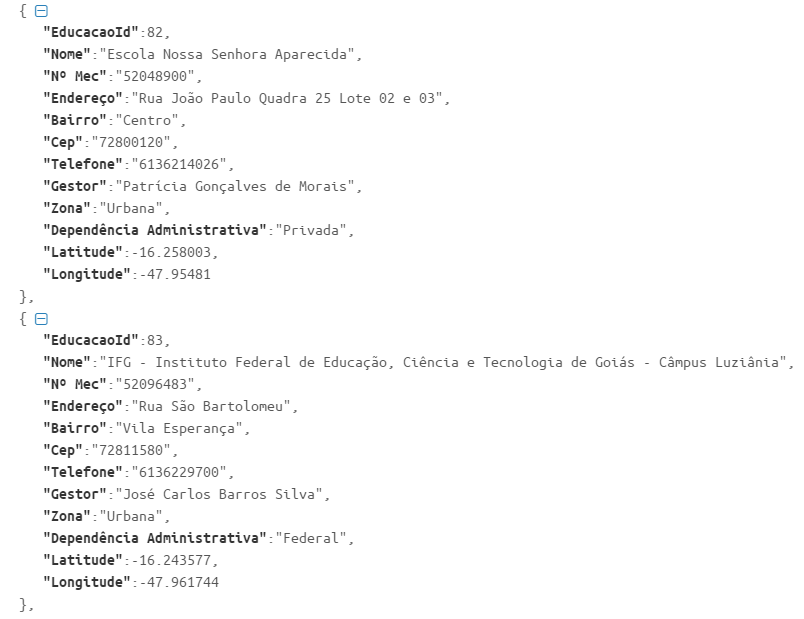
\includegraphics[width=0.75\textwidth]{./img/cap_IV/4-ConsultaJSON}
\caption{Consulta \textit{RESTful} com formato JSON.}
\label{fig:ConsultaJSON}
\end{figure}

A Figura \ref{fig:ConsultaJSON} apresenta o resultado de uma consulta REST no formato JSON. Para realizar chamadas de um serviço \textit{RESTful}, é necessário apenas a passagem de parâmetros (se existirem) através da URL. Por exemplo, pode-se realizar uma consulta das instituições de ensino no SIG Web Luziânia através da URL: \textbf{http://sigluziania/api/mapa/educacao}. Assim, fazendo o uso do mesmo mecanismo usado na utilização de \textit{Web Services}.

\newpage

\section{Interface do SIG Web Luziânia}

O SIG Web Luziânia é composto por duas partes: a georreferenciada (parte inicial) e a área administrativa. Na parte georreferenciada ocorre a visualização dos dados georreferenciados (educação, lazer, saúde e segurança) no mapa. A Figura \ref{fig:PaginaInicial} mostra a página inicial do sistema, composto pela visualização dos dados georreferenciados. Os pontos na cor verde, amarelo, vermelho e azul, representam respectivamente dados sobre educação, lazer saúde e segurança, conforme a legenda apresentada na parte inferior do mapa.

\begin{figure}[h]
\centering
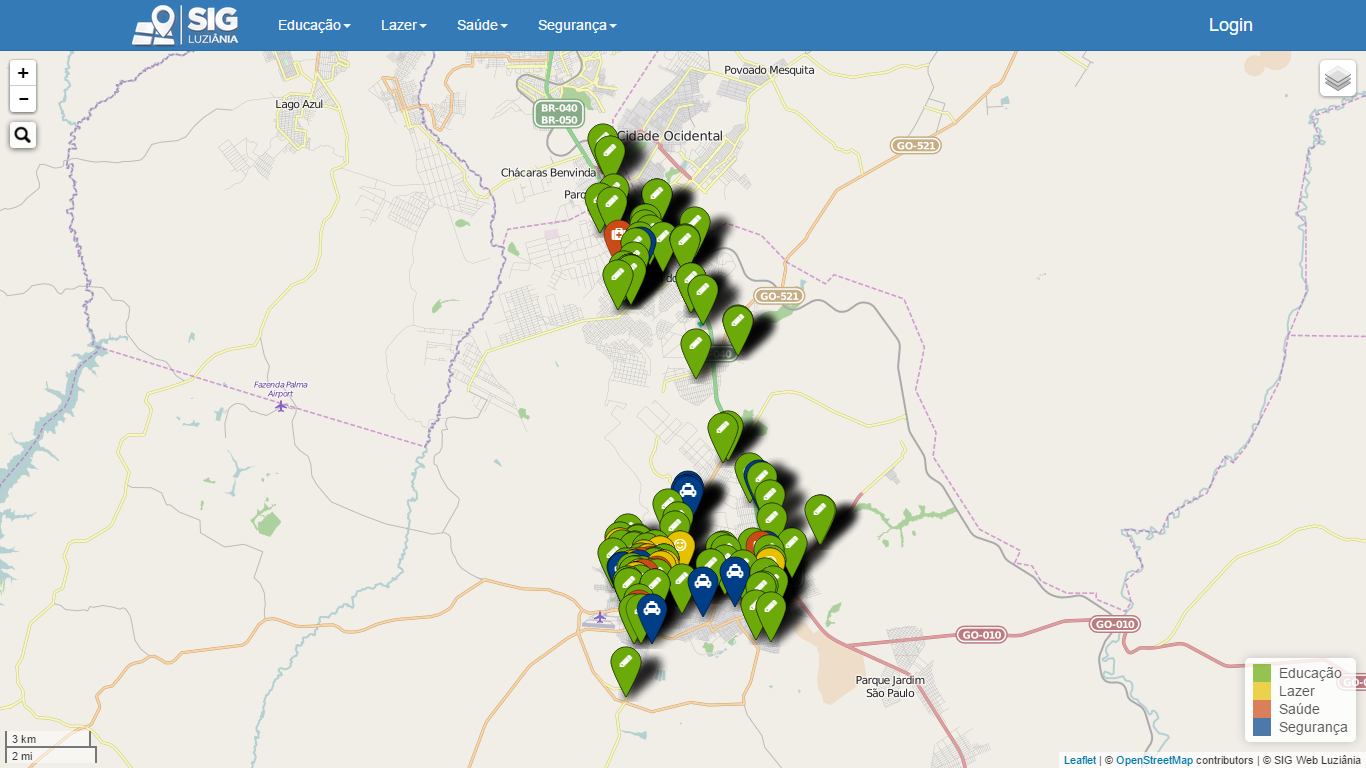
\includegraphics[width=0.80\textwidth]{./img/cap_IV/5-PaginaInicial}
\caption{Página inicial do SIG Web Luziânia.}
\label{fig:PaginaInicial}
\end{figure}

\newpage

Na página inicial do sistema é possível interagir com o mapa. A Figura \ref{fig:BalaoInformacoes} mostra a interação com a visualização dos dados representados no mapa, onde a partir do clique do \textit{mouse} é possível visualizar informações do ponto desejado. A Figura \ref{fig:Camadas} apresenta as camadas representadas no mapa (educação, lazer, saúde e segurança), assim como o tipo de mapa a ser visualizado (rua ou satélite). A Figura \ref{fig:PesquisaMapa} mostra a interação com a parte de pesquisa dos dados do mapa. Ainda é possível interagir com o mapa através do \textit{zoom}.

\begin{figure}[h]
\centering
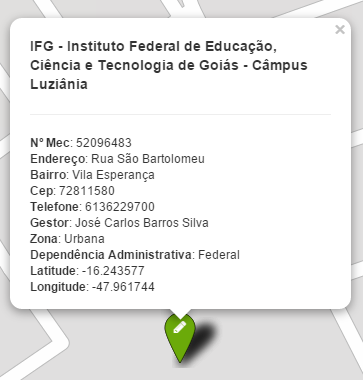
\includegraphics[width=0.36\textwidth]{./img/cap_IV/6-BalaoInformacoes}
\caption{Balão de informações.}
\label{fig:BalaoInformacoes}
\end{figure}

\begin{figure}[h]
\centering
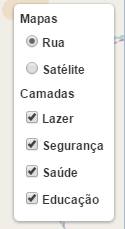
\includegraphics[width=0.14\textwidth]{./img/cap_IV/7-Camadas}
\caption{Camadas do mapa.}
\label{fig:Camadas}
\end{figure}

\begin{figure}[h]
\centering
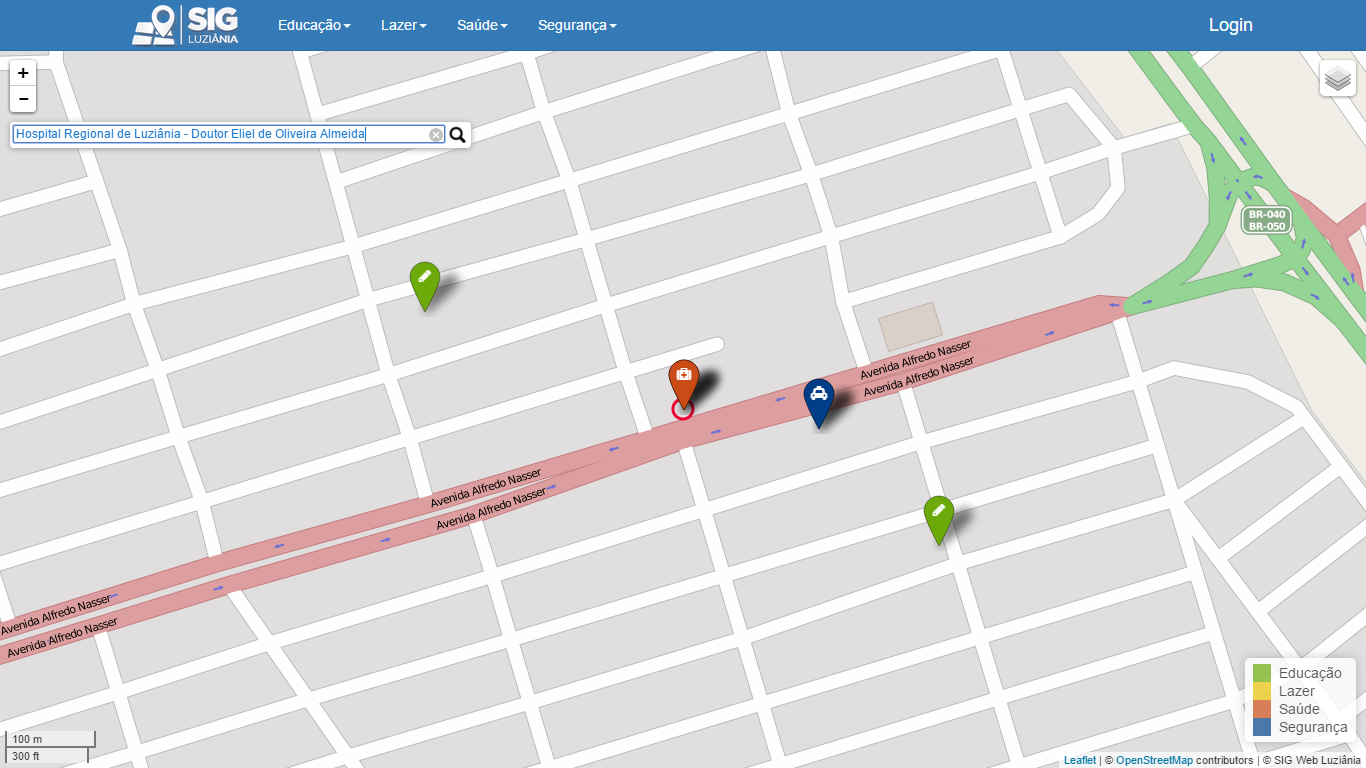
\includegraphics[width=0.80\textwidth]{./img/cap_IV/8-PesquisaMapa}
\caption{Interação com a pesquisa no mapa.}
\label{fig:PesquisaMapa}
\end{figure}

\newpage

Ainda na parte inicial do sistema é apresentado menus onde todos os dados apresentados no mapa são organizados e visualizados. A Figura \ref{fig:Instituicoes} apresenta o menu “Educação”, onde ocorre a visualização dos dados sobre as instituições de ensino, assim como gráficos representando as notas das instituições e suas evoluções no IDEB e ENEM, apresentadas nas Figuras \ref{fig:IDEBInicial}, \ref{fig:IDEBFinal} e \ref{fig:ENEM}.

\begin{figure}[h]
\centering
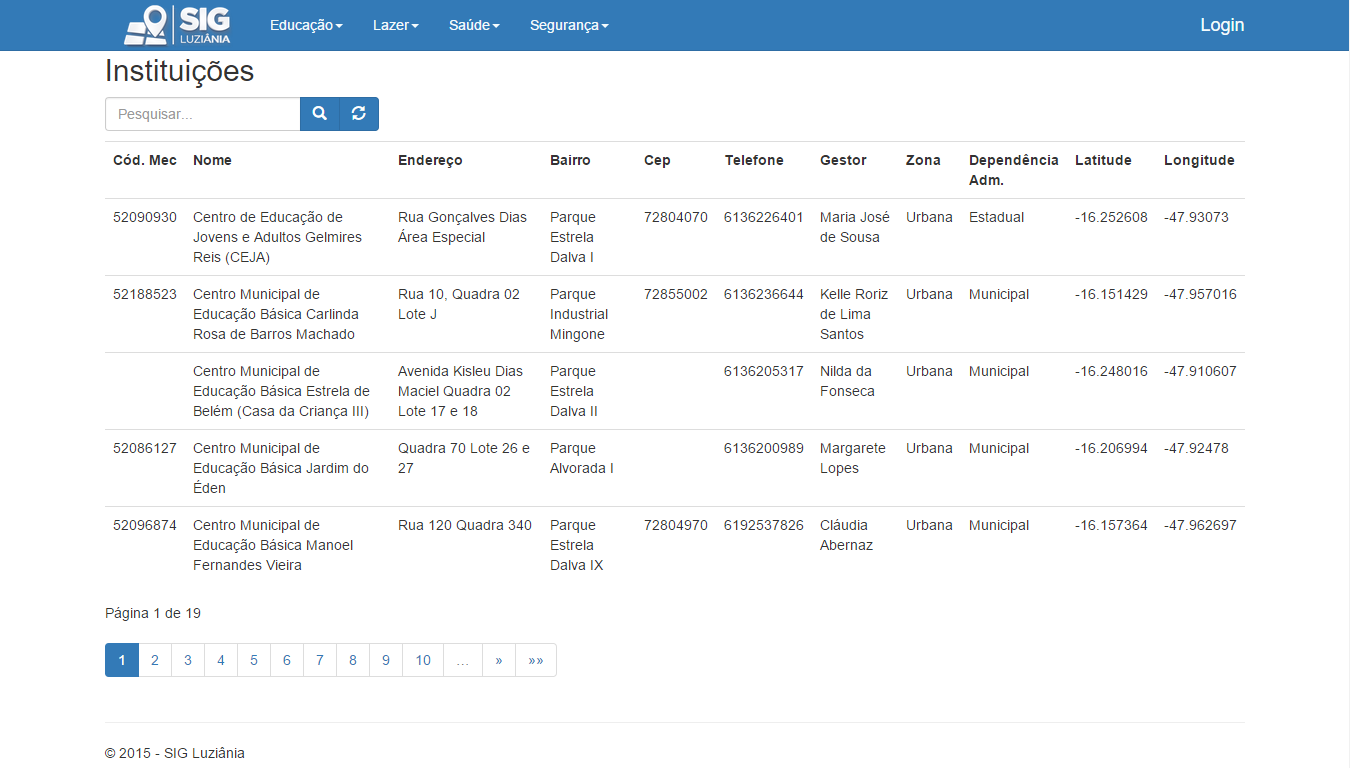
\includegraphics[width=0.80\textwidth]{./img/cap_IV/9-Instituicoes}
\caption{Instituições de ensino.}
\label{fig:Instituicoes}
\end{figure}

\begin{figure}[h]
\centering
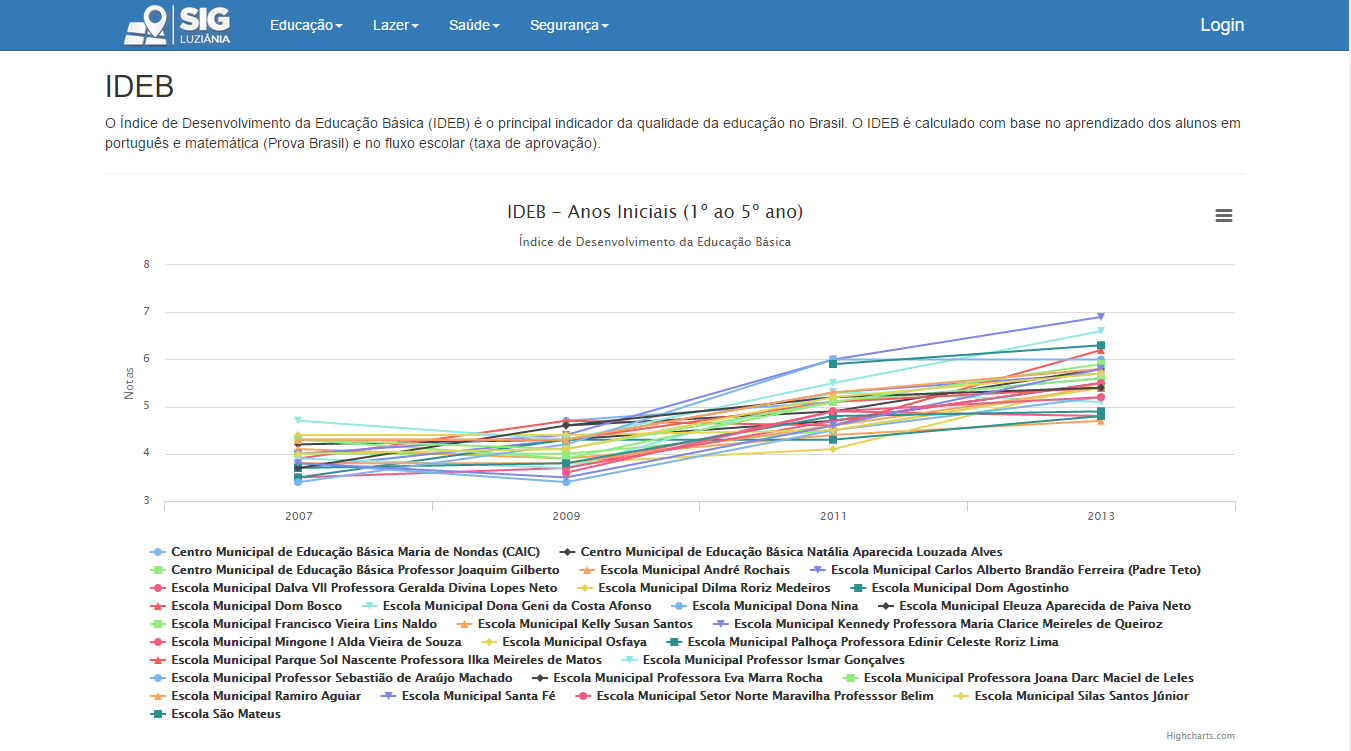
\includegraphics[width=0.80\textwidth]{./img/cap_IV/10-IDEBInicial}
\caption{Notas do IDEB anos iniciais.}
\label{fig:IDEBInicial}
\end{figure}

\newpage

\begin{figure}[h]
\centering
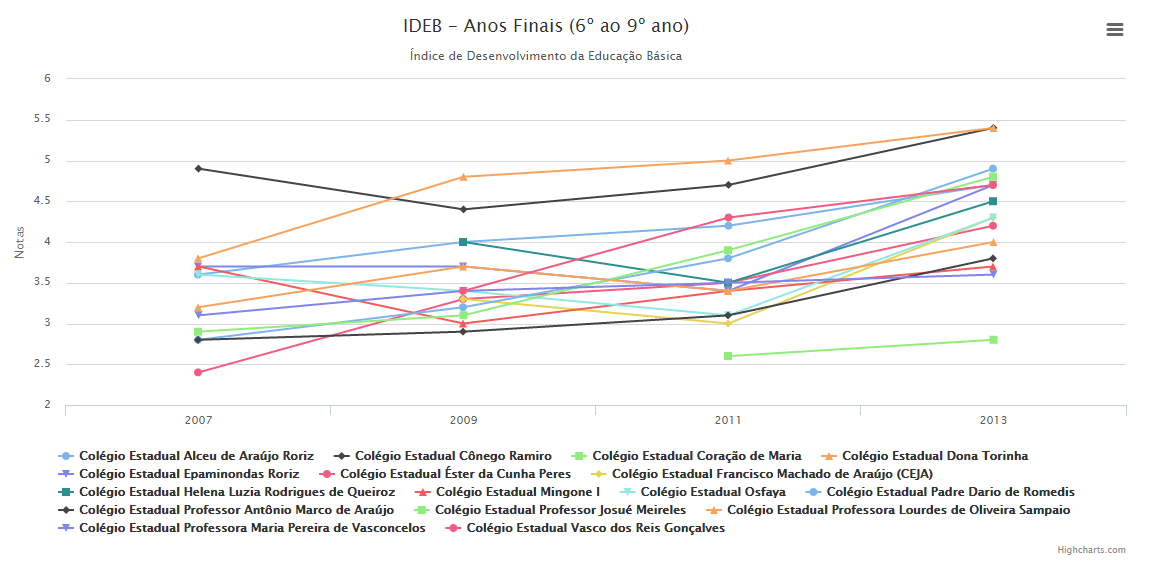
\includegraphics[width=0.80\textwidth]{./img/cap_IV/11-IDEBFinal}
\caption{Notas do IDEB anos finais.}
\label{fig:IDEBFinal}
\end{figure}

\begin{figure}[h]
\centering
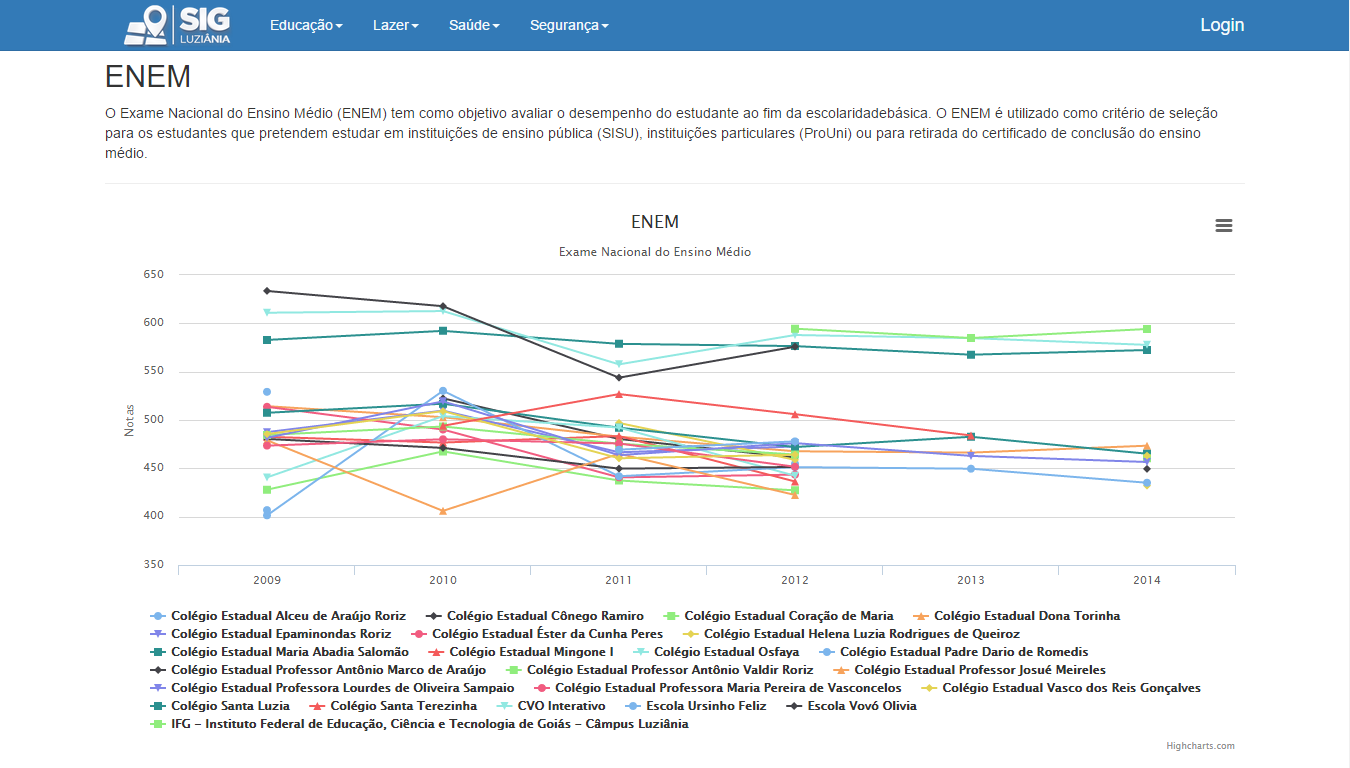
\includegraphics[width=0.80\textwidth]{./img/cap_IV/12-ENEM}
\caption{Notas do ENEM.}
\label{fig:ENEM}
\end{figure}

A Figura \ref{fig:Lazer} é apresentado o menu “Lazer”, contendo as localidades de entretenimento. O menu “Saúde” contém as localidades de saúde, apresentada na Figura \ref{fig:Saude}. A Figura \ref{fig:Especialidade}, apresenta as especialidades presente nas localidades de saúde.

\begin{figure}[h]
\centering
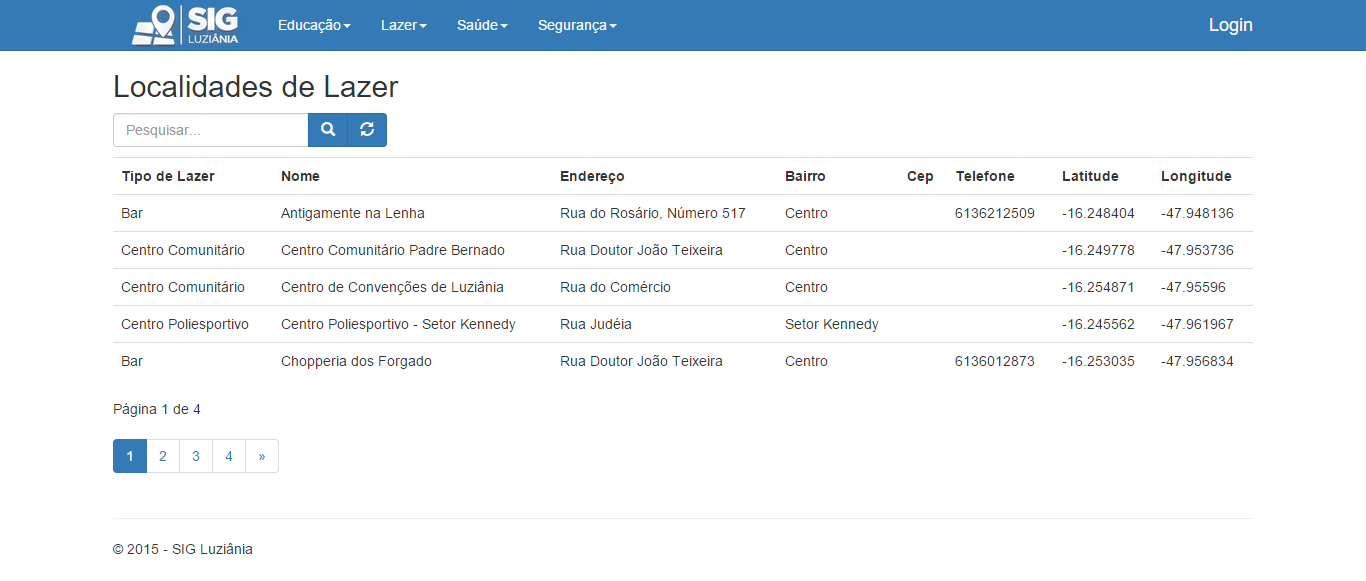
\includegraphics[width=0.80\textwidth]{./img/cap_IV/13-Lazer}
\caption{Localidades de entretenimento.}
\label{fig:Lazer}
\end{figure}

\begin{figure}[h]
\centering
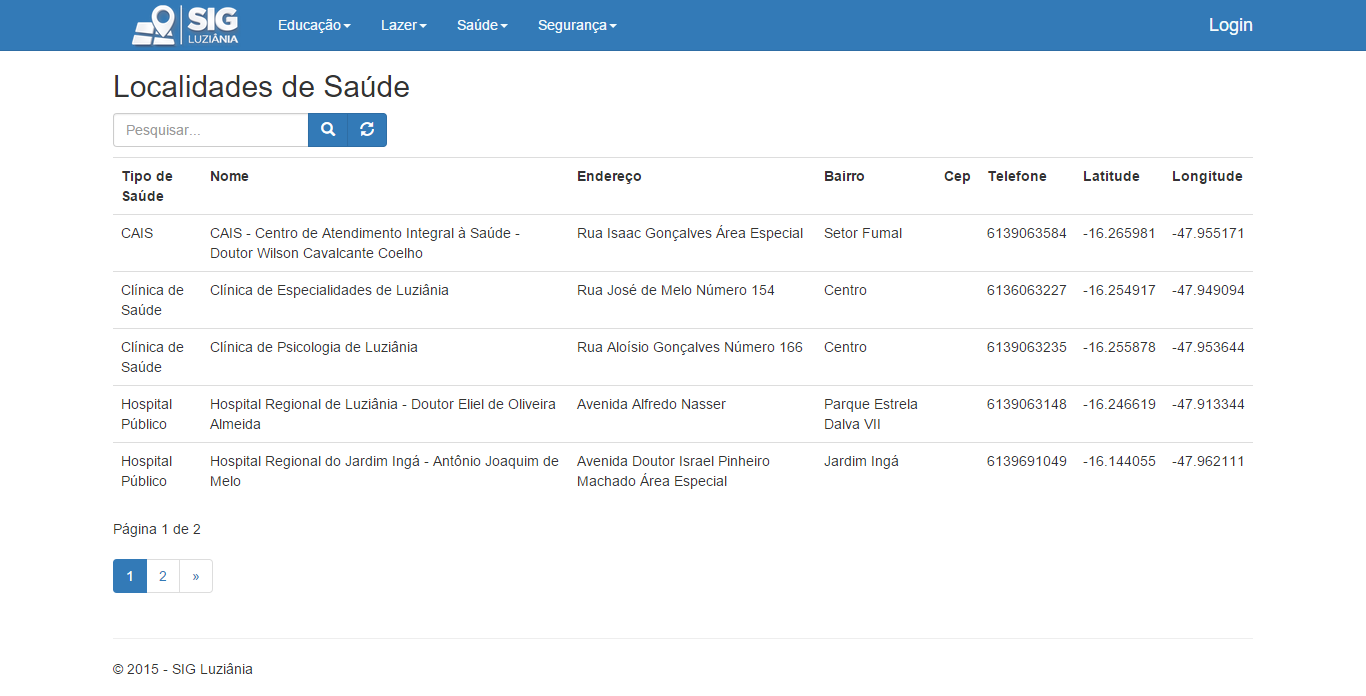
\includegraphics[width=0.80\textwidth]{./img/cap_IV/14-Saude}
\caption{Localidades de saúde.}
\label{fig:Saude}
\end{figure}

\newpage

\begin{figure}[h]
\centering
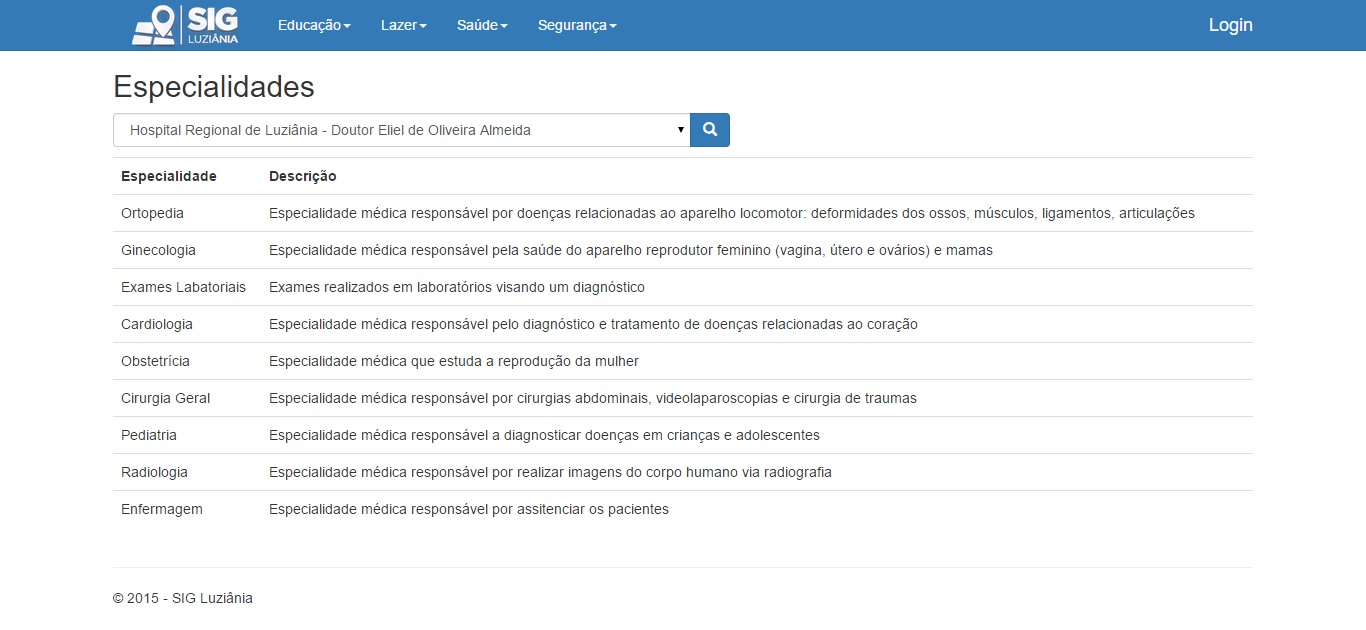
\includegraphics[width=0.80\textwidth]{./img/cap_IV/15-Especialidades}
\caption{Especialidades de saúde.}
\label{fig:Especialidade}
\end{figure}

\newpage

E por fim, no menu “Segurança” é apresentado as localidades de segurança apresentadas na Figura \ref{fig:Seguranca}.

\begin{figure}[h]
\centering
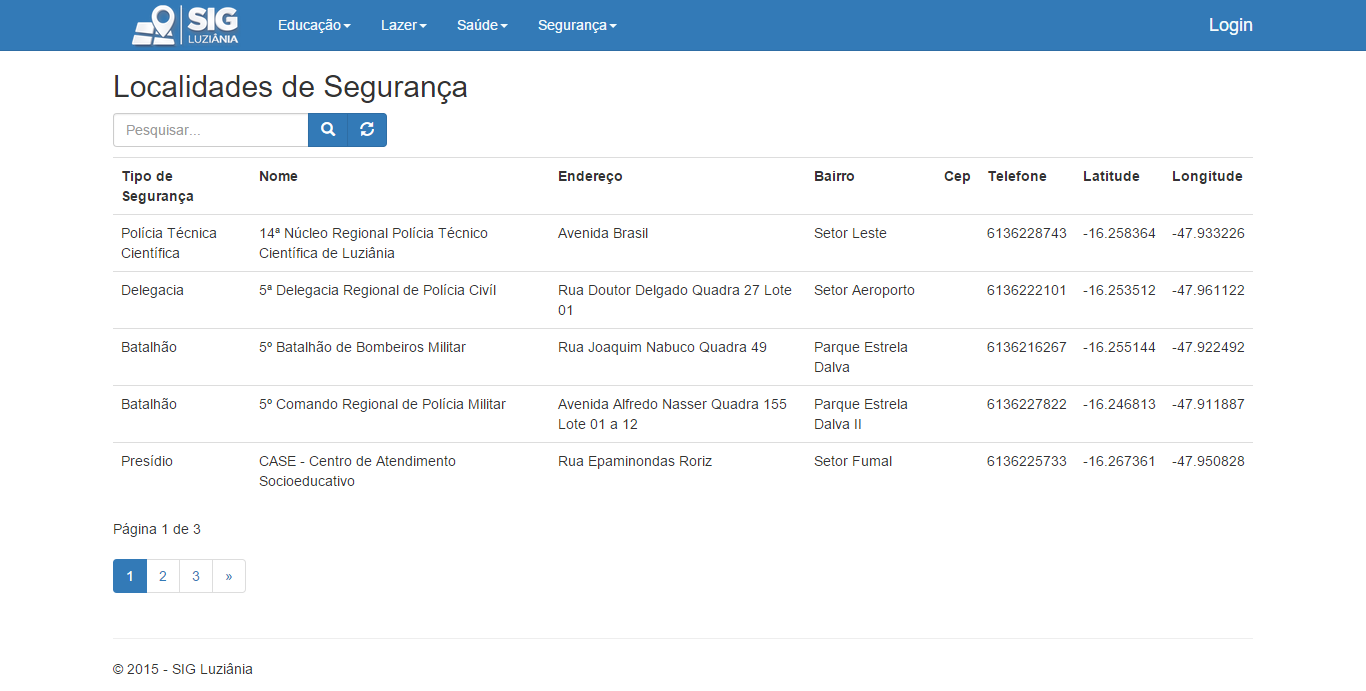
\includegraphics[width=0.80\textwidth]{./img/cap_IV/16-Seguranca}
\caption{Localidades de segurança.}
\label{fig:Seguranca}
\end{figure}

A área administrativa do sistema é responsável pelo acesso e controle dos dados apresentados no mapa. A Figura \ref{fig:Login} exibe a tela de \textit{login} do SIG Web Luziânia para acesso a área administrativa do sistema.

\begin{figure}[h]
\centering
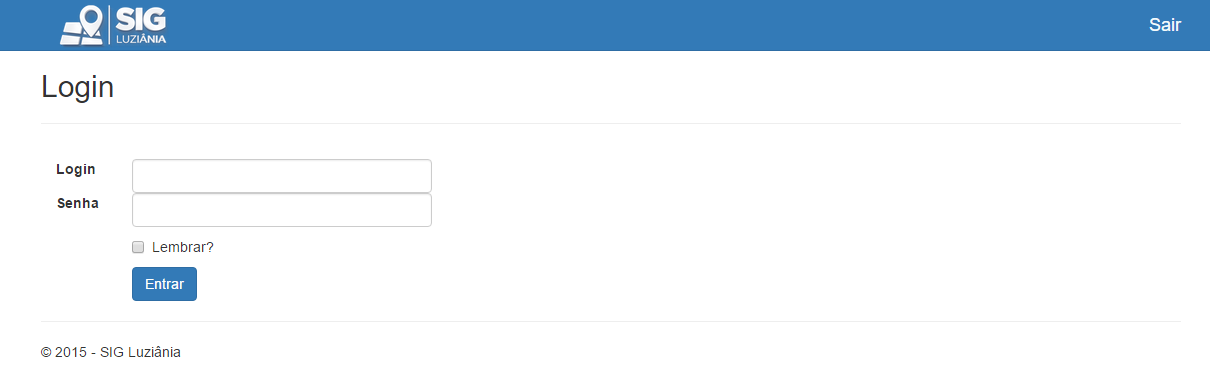
\includegraphics[width=0.80\textwidth]{./img/cap_IV/17-Login}
\caption{Tela de \textit{login}.}
\label{fig:Login}
\end{figure}

Após efetuado o \textit{login} pelo usuário é visualizado a tela da área administrativa, responsável pelo controle dos dados do SIG Web Luziânia, apresentado pela Figura \ref{fig:AreaAdministrativa}.  A área administrativa é composta pelos respectivos menus:

\begin{itemize}
\item “Administrador”: responsável por gerenciar os administradores do sistema;
\item “Educação”: responsável por gerenciar as instituições de ensino e suas avaliações;
\item “Lazer”: responsável por gerenciar as localidades de entretenimento e seus tipos de entretenimento;
\item “Saúde”: responsável por gerenciar as localidades de saúde, tipos de localidades e especialidades;
\item “Segurança”: responsável por gerenciar todas as localidades de segurança e seus tipos de localidades.
\end{itemize}

\newpage

\begin{figure}[h]
\centering
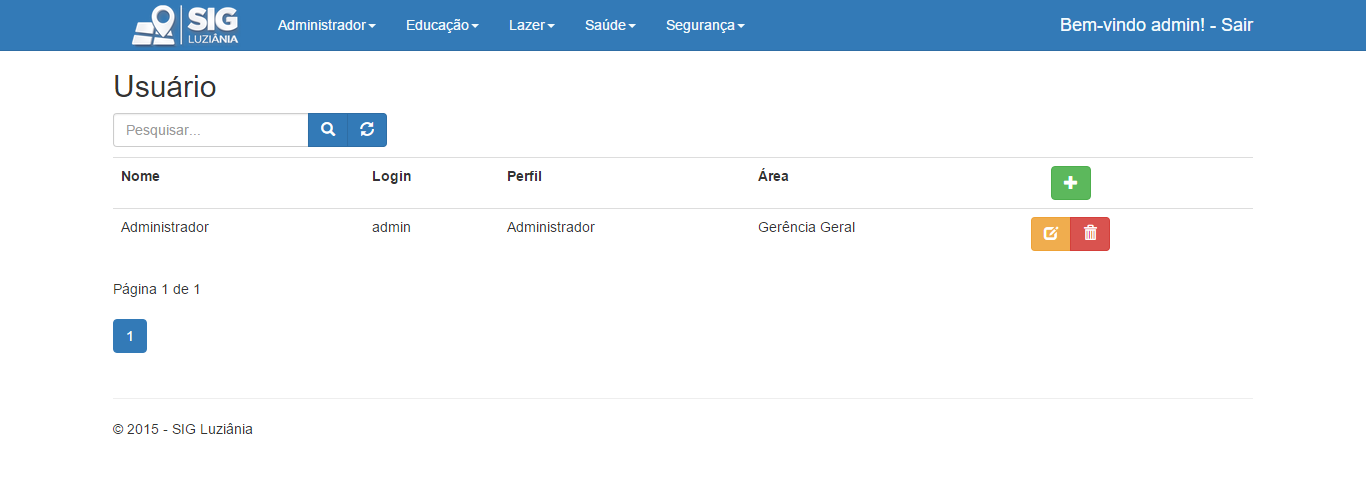
\includegraphics[width=0.80\textwidth]{./img/cap_IV/18-AreaAdministrativa}
\caption{Área administrativa do sistema.}
\label{fig:AreaAdministrativa}
\end{figure}

As Figuras \ref{fig:AdmEducacao}, \ref{fig:AdmLazer}, \ref{fig:AdmSaude} e \ref{fig:AdmSeguranca} apresentam a área de controle de dados dos menus: “Educação”, “Lazer”, “Saúde” e “Segurança”.

\begin{figure}[h]
\centering
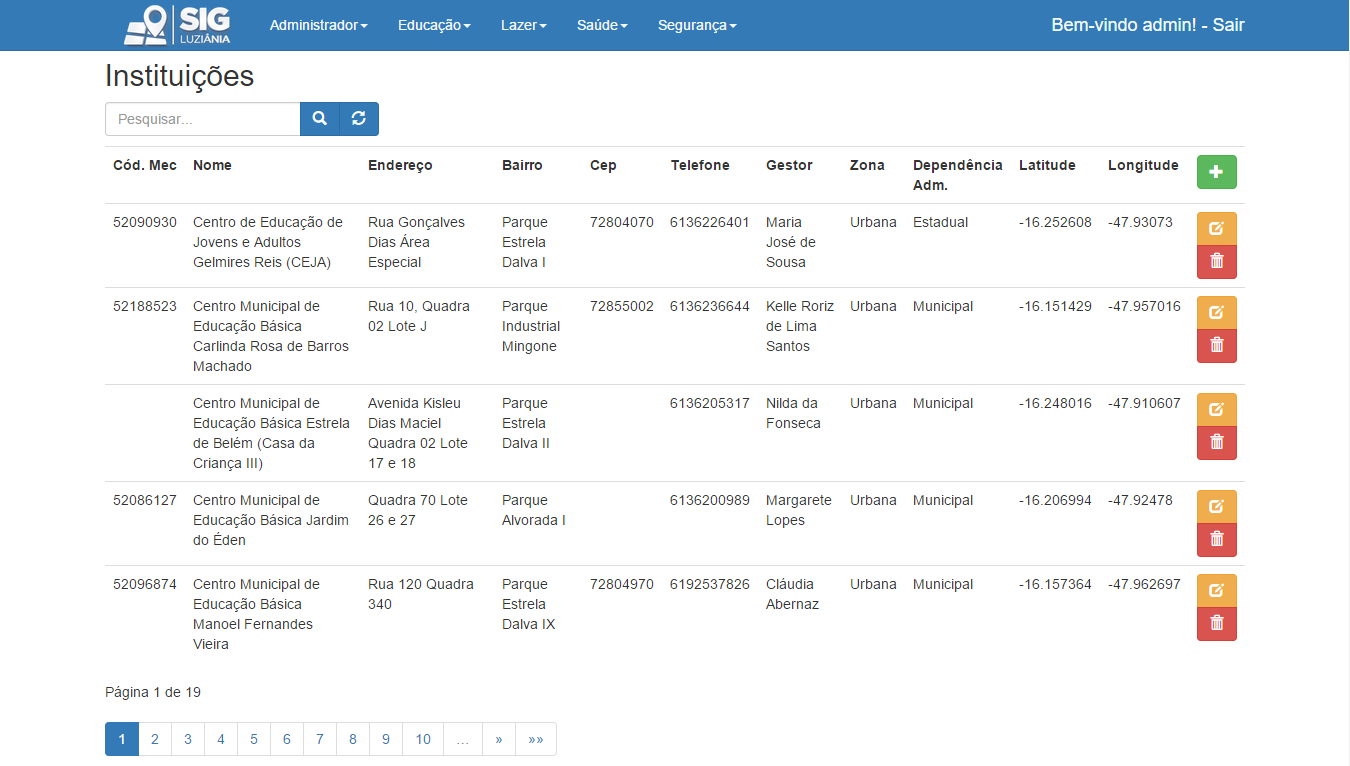
\includegraphics[width=0.80\textwidth]{./img/cap_IV/19-AdmEducacao}
\caption{Área administrativa dos dados de educação.}
\label{fig:AdmEducacao}
\end{figure}

\begin{figure}[h]
\centering
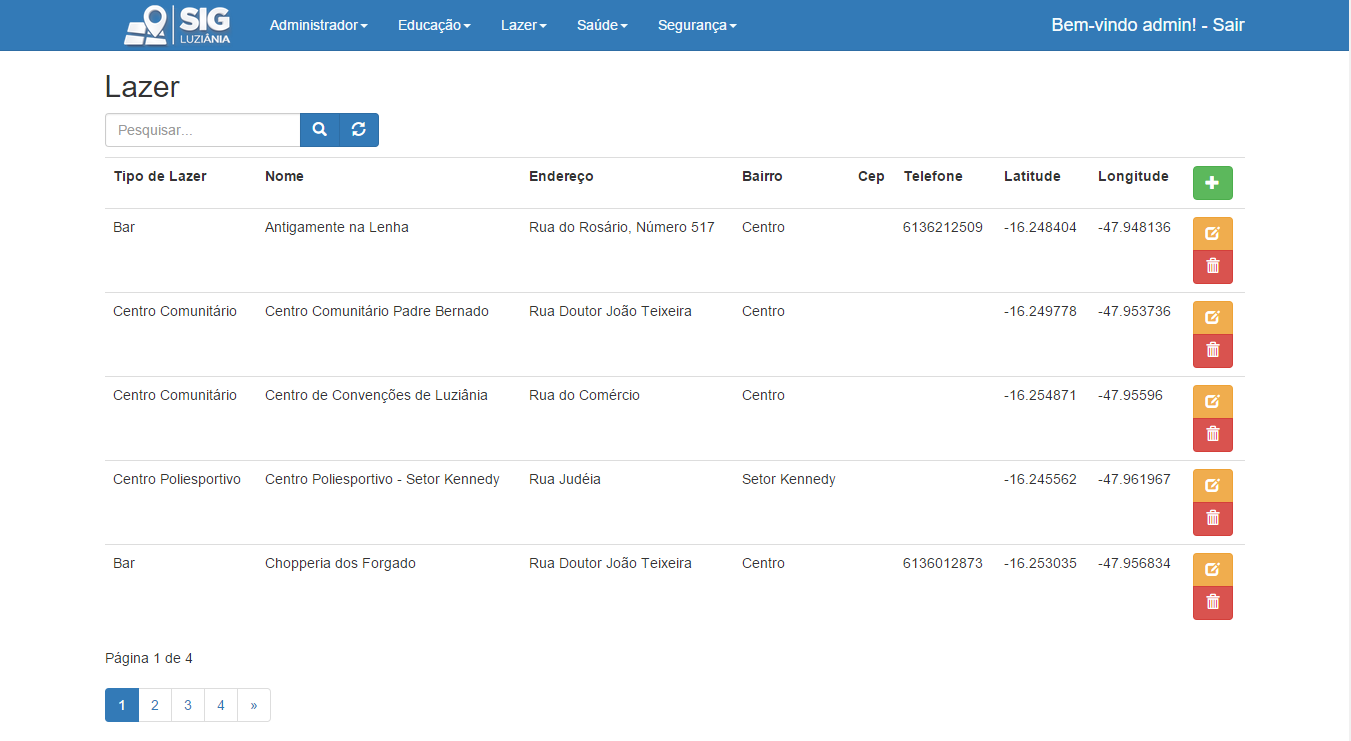
\includegraphics[width=0.80\textwidth]{./img/cap_IV/20-AdmLazer}
\caption{Área administrativa dos dados de entretenimento.}
\label{fig:AdmLazer}
\end{figure}

\newpage

\begin{figure}[h]
\centering
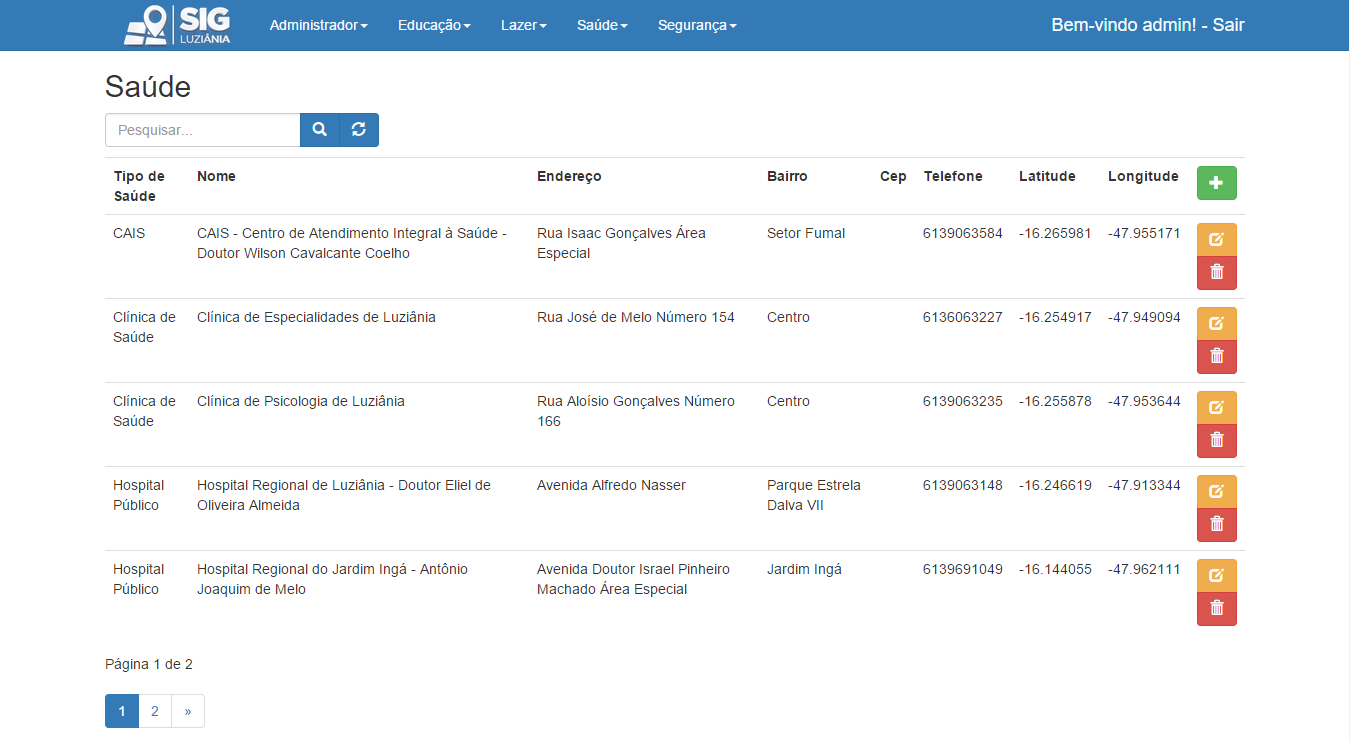
\includegraphics[width=0.80\textwidth]{./img/cap_IV/21-AdmSaude}
\caption{Área administrativa dos dados de saúde.}
\label{fig:AdmSaude}
\end{figure}

\begin{figure}[h]
\centering
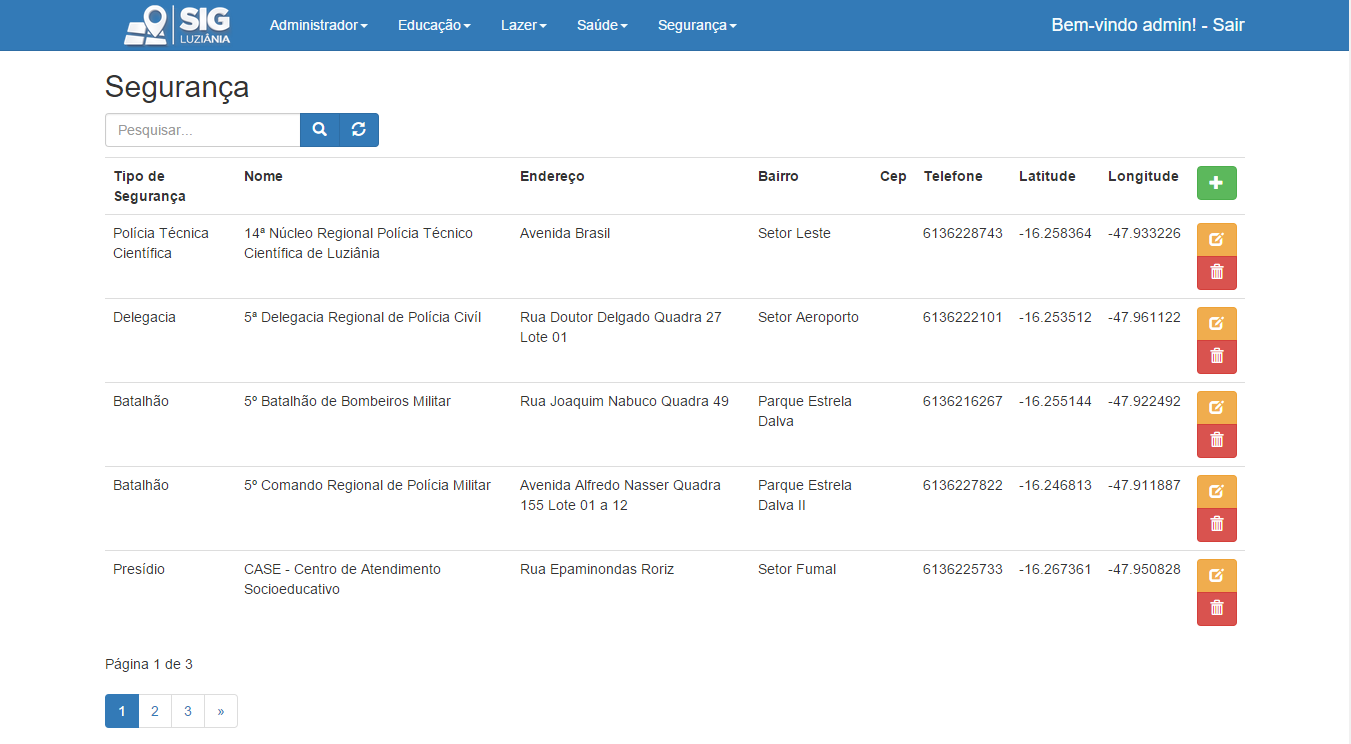
\includegraphics[width=0.80\textwidth]{./img/cap_IV/22-AdmSeguranca}
\caption{Área administrativa dos dados de segurança.}
\label{fig:AdmSeguranca}
\end{figure}

\newpage

As Figuras \ref{fig:AdmAvaliacao} e \ref{fig:AdmEspecialidade} apresentam os controles de dados das avaliações e especialidades presentes respectivamente nos menus de "Educação" e "Saúde". Nessa área do sistema é realizado o vínculo das avaliações com as instituições de ensino e as especialidades com as instituições de saúde.

\begin{figure}[h]
\centering
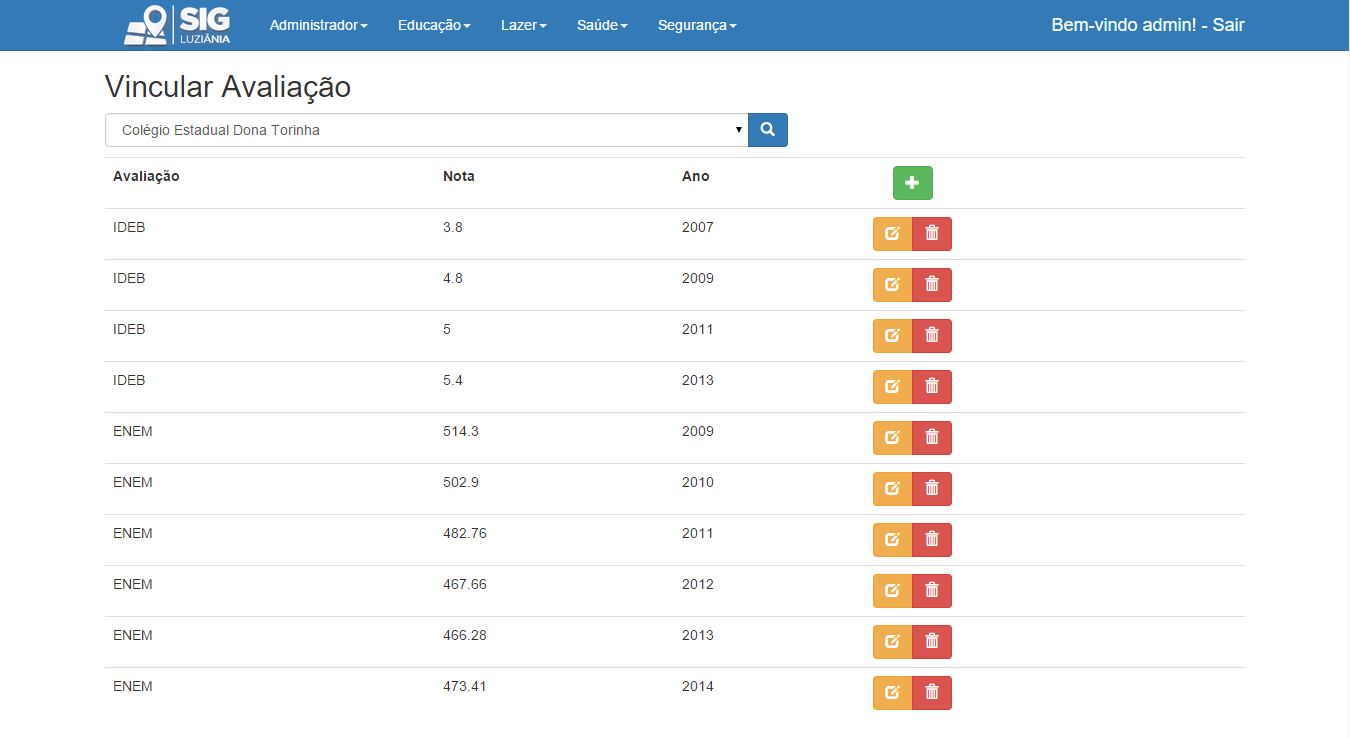
\includegraphics[width=0.80\textwidth]{./img/cap_IV/23-AdmAvaliacao}
\caption{Área administrativa de avaliações.}
\label{fig:AdmAvaliacao}
\end{figure}

\newpage

\begin{figure}[h]
\centering
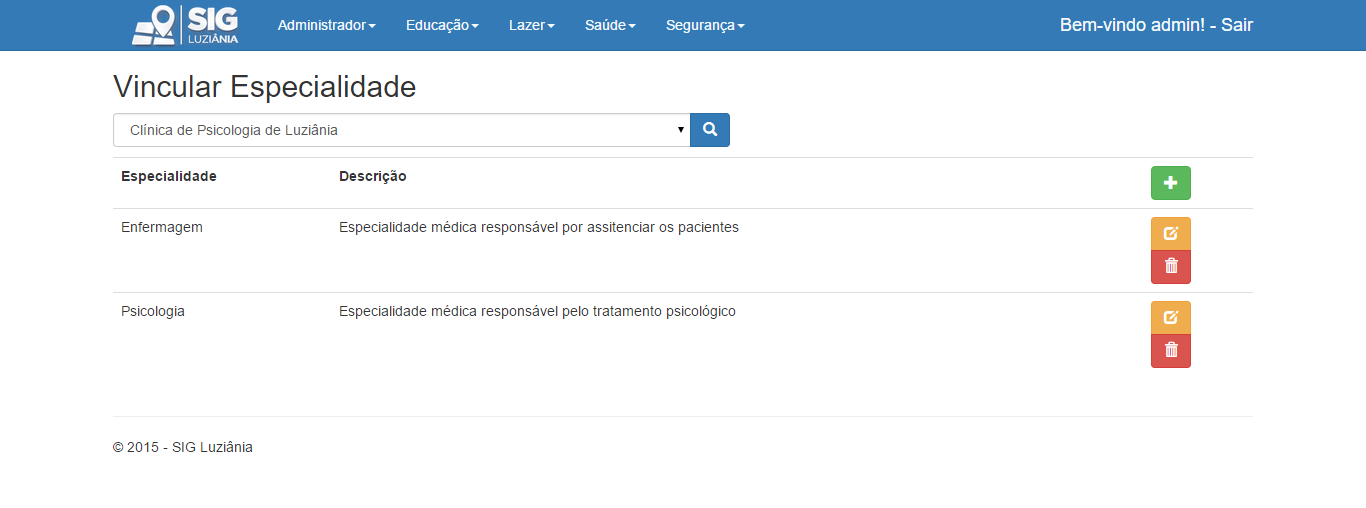
\includegraphics[width=0.80\textwidth]{./img/cap_IV/24-AdmEspecialidade}
\caption{Área administrativa de especialidades.}
\label{fig:AdmEspecialidade}
\end{figure}

Em toda a área administrativa do sistema, é realizado todas as operações de controle de dados (inserir, visualizar, atualizar e excluir). As operações de inserir, atualizar e excluir estão presentes em \textit{pop-up’s} presente em todos os menus do sistema. A Figura \ref{fig:AdmAdicionar}, \ref{fig:AdmEditar} e \ref{fig:AdmExcluir} representam respectivamente cada uma das operações no menu “Saúde”.

\begin{figure}[h]
\centering
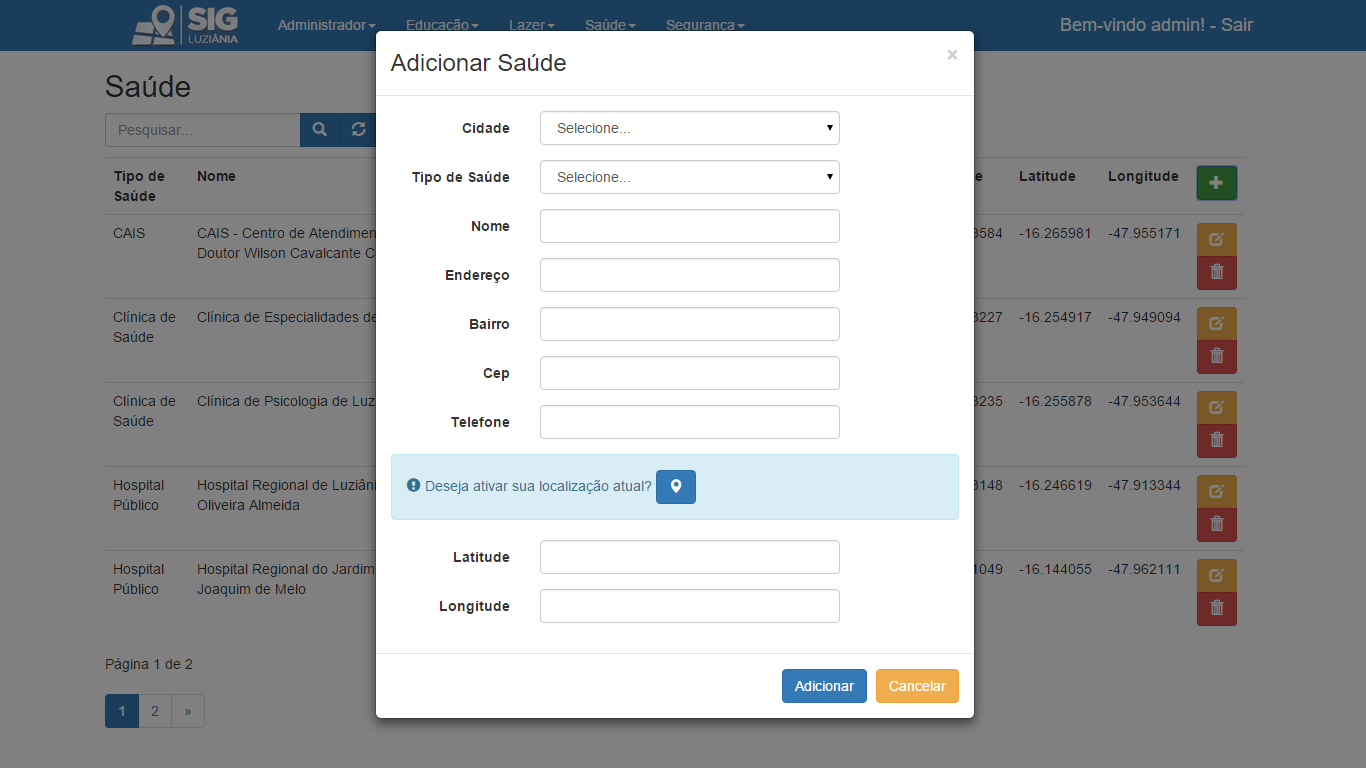
\includegraphics[width=0.80\textwidth]{./img/cap_IV/25-AdmAdicionar}
\caption{\textit{Pop-up} para adicionar localidade de saúde.}
\label{fig:AdmAdicionar}
\end{figure}

\newpage

\begin{figure}[h]
\centering
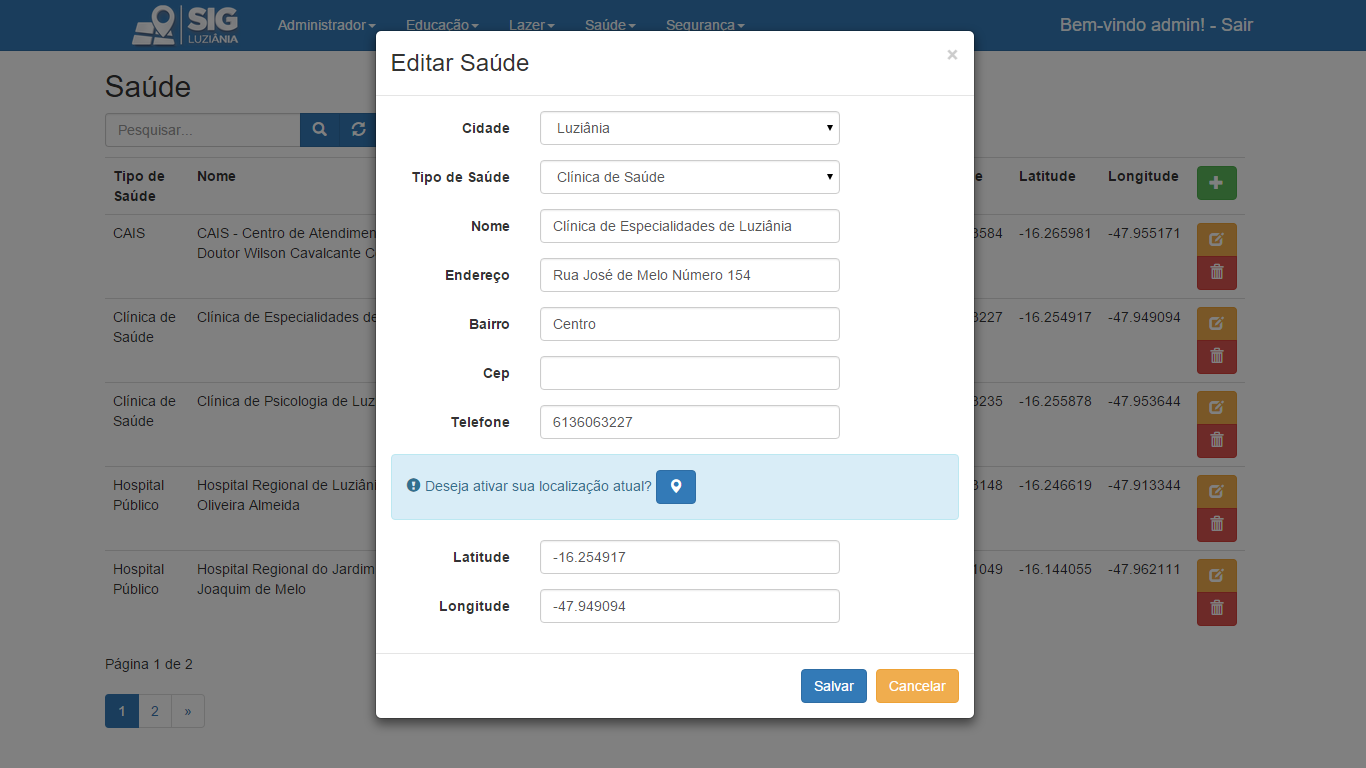
\includegraphics[width=0.80\textwidth]{./img/cap_IV/26-AdmEditar}
\caption{\textit{Pop-up} para editar localidade de saúde.}
\label{fig:AdmEditar}
\end{figure}

\begin{figure}[h]
\centering
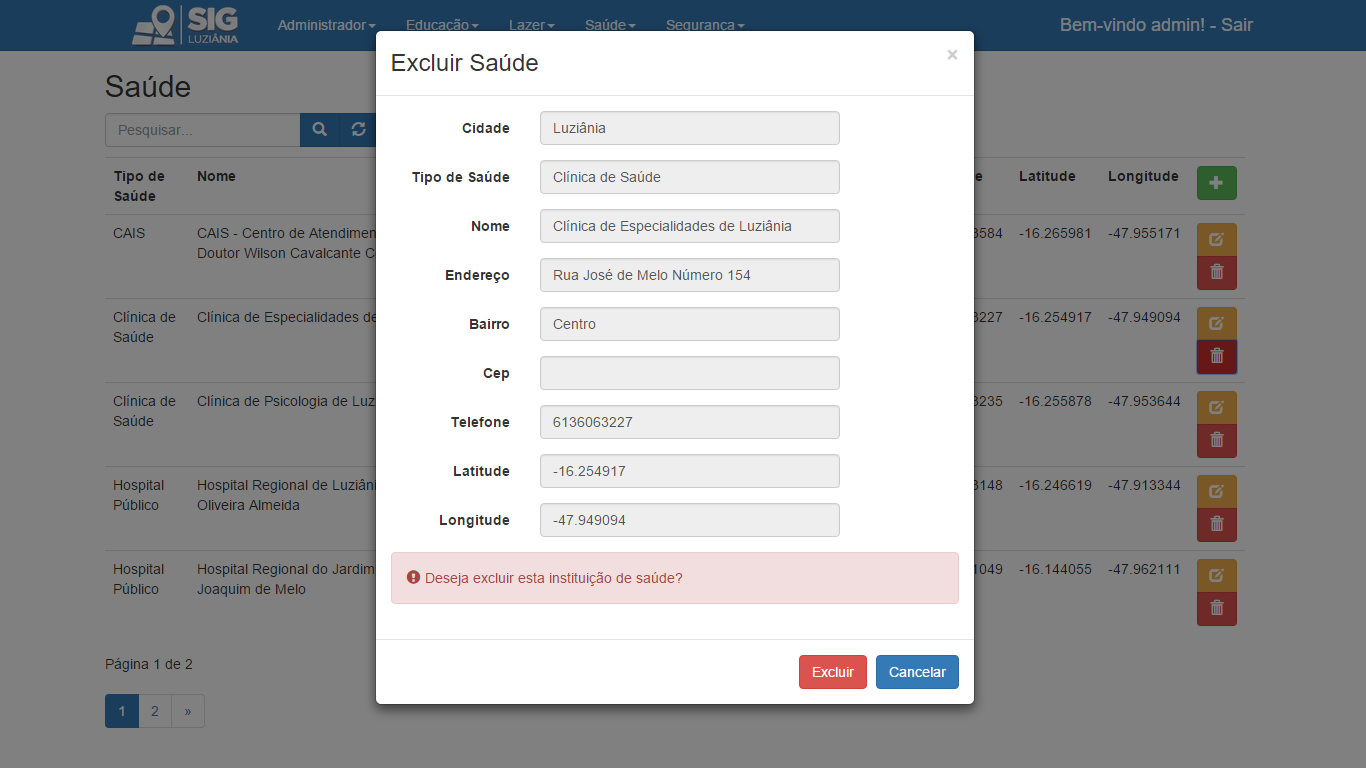
\includegraphics[width=0.80\textwidth]{./img/cap_IV/27-AdmExcluir}
\caption{\textit{Pop-up} para excluir localidade de saúde.}
\label{fig:AdmExcluir}
\end{figure}

O SIG Web Luziânia foi construído utilizando as tecnologias Web mais recentes como o HTML5, \textit{Cascading Style Sheets 3} (CSS3) e Javascript. Por esse motivo, o sistema é totalmente responsível e acessível em dispositivos móveis. A Figura \ref{fig:MobileMapa} e a Figura \ref{fig:MobileAdm} apresentam essa acessibilidade.

\begin{figure}[h]
\centering
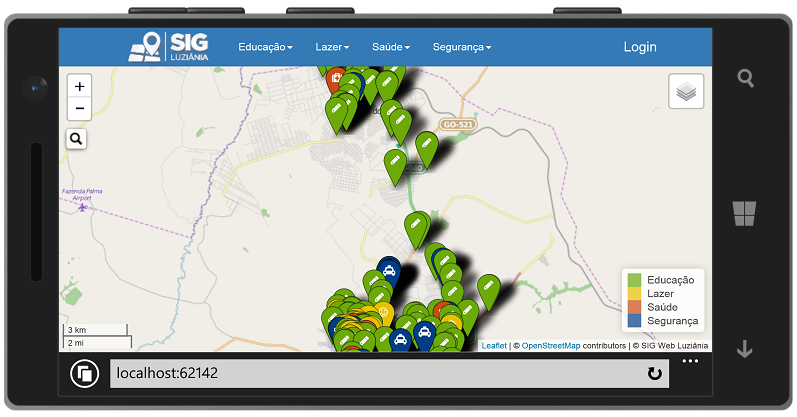
\includegraphics[width=0.80\textwidth]{./img/cap_IV/28-MobileMapa}
\caption{Visualização da página inicial do sistema em um \textit{Smartphone}.}
\label{fig:MobileMapa}
\end{figure}

\newpage

\begin{figure}[h]
\centering
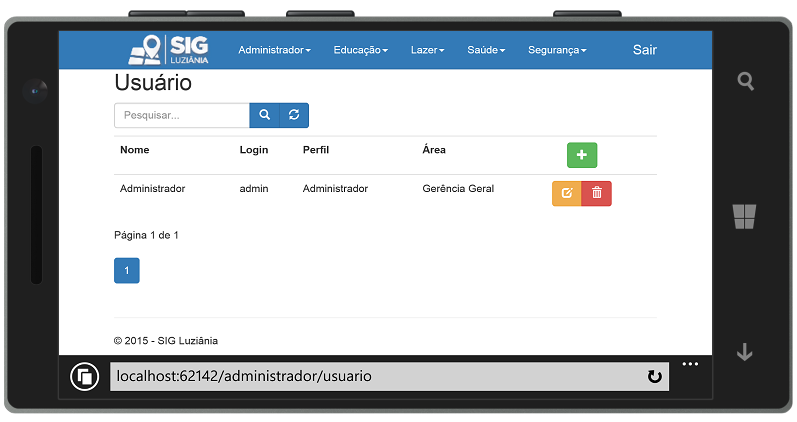
\includegraphics[width=0.80\textwidth]{./img/cap_IV/29-MobileAdm}
\caption{Visualização da área administrativa do sistema em um \textit{Smartphone}.}
\label{fig:MobileAdm}
\end{figure}

\section{Trabalhos Relacionados}

A grande extensão do território brasileiro em conjunto com sua população, torna o uso de um SIG para o gerenciamento das informações fundamental, seja no âmbito municipal, estadual e federal. Grandes cidades brasileiras possuem SIGs Web para o gerenciamento e visualização das informações de uma maneira pública a população.

Como SIGs Web relacionados a este trabalho temos: Sistema de Informação Geográfica de Goiânia (SIGGO), Sistema de Informação Geográfica da Bahia (SIG Bahia) e o Sistema Municipal de Informações Urbanas (SIURB).

\newpage

O SIGGO \cite{siggo} apresenta informações da cidade de Goiânia, a Figura \ref{fig:SIGGO} apresenta a página inicial do sistema. Através do SIGGO é possível obter as seguintes informações:

\begin{itemize}
\item Bairros, quadras e lotes;
\item Ruas, praças e avenidas;
\item Hidrografia;
\item Escolas;
\item Unidades de saúde.
\end{itemize}

\begin{figure}[h]
\centering
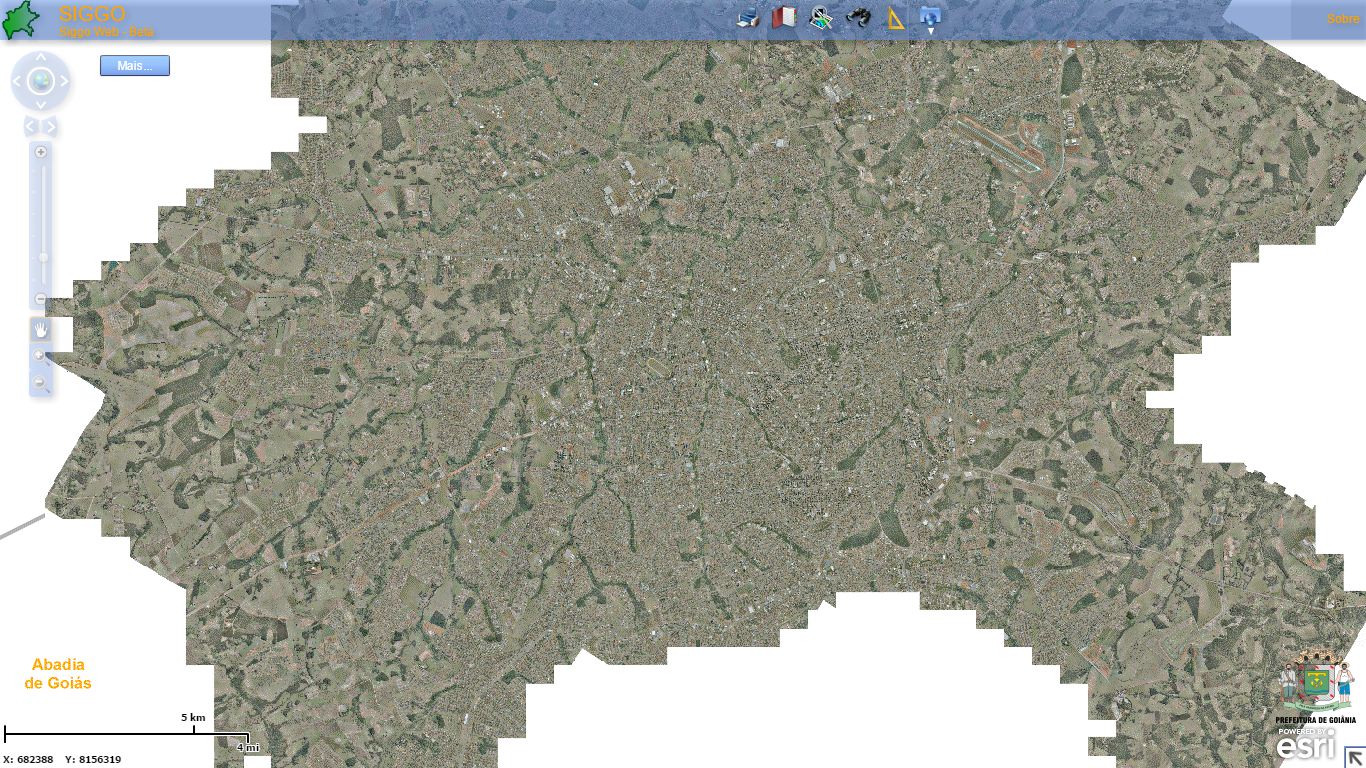
\includegraphics[width=0.80\textwidth]{./img/cap_IV/30-SIGGO}
\caption{Página inicial do SIGGO.}
\label{fig:SIGGO}
\end{figure}

O SIG Bahia \cite{sigbahia} apresenta informações do estado da Bahia, a Figura \ref{fig:SIGBahia} apresenta a página inicial do sistema. O SIG Bahia apresenta um grande número de informações disponíveis, as principais são:

\begin{itemize}
\item Hidrografia;
\item Sistema de transporte;
\item Rodoviais, estradas, ferroviais;
\item Biodiversidade;
\item Unidades de conservações;
\item Mapas sociais;
\item Mapas geológicos.
\end{itemize}

\newpage

\begin{figure}[h]
\centering
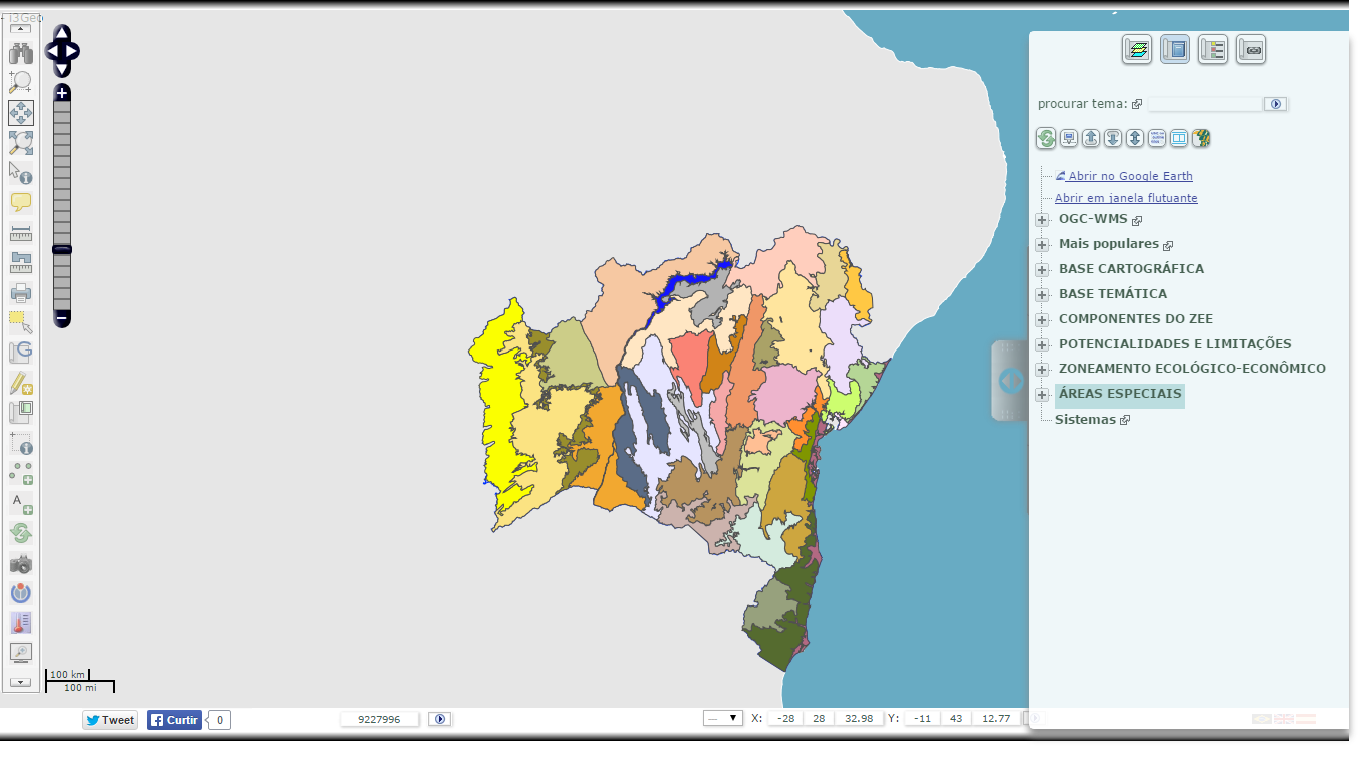
\includegraphics[width=0.80\textwidth]{./img/cap_IV/31-SIGBahia}
\caption{Página inicial SIG Bahia.}
\label{fig:SIGBahia}
\end{figure}

Por fim, o SIURB \cite{siurg} é utilizado na tomada de decisão da administração municipal do município do Rio de Janeiro. A Figura \ref{fig:SIURB} apresenta a página inicial do SIURB.

\begin{figure}[h]
\centering
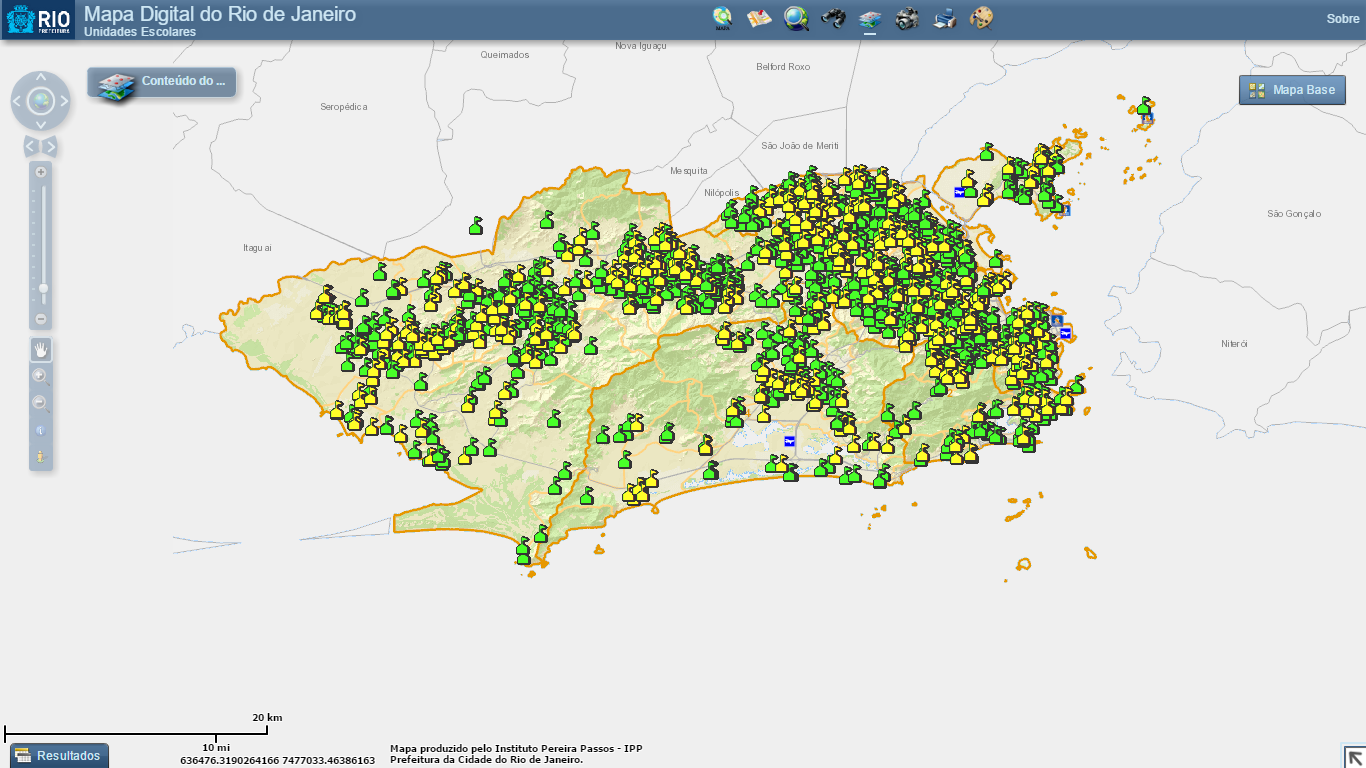
\includegraphics[width=0.80\textwidth]{./img/cap_IV/32-SIURB}
\caption{Página inicial do SIURB.}
\label{fig:SIURB}
\end{figure}

As principais informações disponíveis no sistema são:

\begin{itemize}
\item Ações da prefeitura nas áreas pacificadas;
\item Segurança;
\item Transporte público;
\item Saúde;
\item Educação;
\item Lazer e cultura.
\end{itemize}

A principal característica presente nos SIGs Web citados e no SIG Web Luziânia é tornar a tomada de decisão mais ágil e precisa para os gestores que utilizam o sistema. A grande diferença é a utilização da tecnologia \textit{Adobe Flex} na interface no sistema. Essa tecnologia impossibilita que o sistema seja responsível em dispositivos móveis, tornando a interface pouco amigável ao usuário. O uso de tecnologias como HTML5, CSS3 e Javascript se faz essencial para que o SIG Web esteja disponível em dispositivos móveis, como ocorre no SIG Web Luziânia.